
\documentclass[11pt,a4paper,headsepline,bibliography=totoc,idxtotoc,DIV12,openright,twoside=true,chapterprefix=on]{scrbook} %draft zum Schluss
\renewcommand*{\chapterheadstartvskip}{\vspace*{5cm}} %rausnehmen scrbook
% optional: oneside
%\pagestyle{myheadings}

%\markright{Basics}
\addtokomafont{pageheadfoot}{\linespread{1}\selectfont}
%\usepackage[T1]{fontenc} % Windows
\usepackage{ucs}
\usepackage[rflt]{floatflt}
\usepackage[german]{babel}
\usepackage{siunitx}
\usepackage{color}
%\usepackage[latin1]{inputenc} % Windows
\usepackage[utf8x]{inputenc}
\usepackage{ulem}
\usepackage{amsmath,amssymb}
\usepackage{amsthm}
%\usepackage{mathtools}
%\usepackage[dvips]{graphicx}
\usepackage{graphicx}
%\usepackage[demo]{graphicx}
\usepackage{caption}
\usepackage{subcaption}

\usepackage{bm}

\usepackage{wrapfig}
\usepackage{sidecap}
\usepackage{multirow}
\usepackage{pgf}
\usepackage{tikz}
\usetikzlibrary{arrows,automata}
%\usepackage{pgf}
\usepackage{subfig}
\usepackage[inline]{fixme}
%\usepackage[justification=raggedright,singlelinecheck=false]{caption}
\usepackage{nicefrac}
\usepackage{setspace}
\usepackage{dcolumn}
%\usepackage{ragged2e}
\usepackage{caption}
\captionsetup{format=plain,indention=0cm}
\usepackage[sort,nocompress]{cite}
%\usepackage{achicago}
%\usepackage[authoryear,square]{natbib}
\usepackage{hyperref}
\hypersetup{colorlinks=true, citecolor=black, filecolor=black, linkcolor=black, urlcolor=black}
\onehalfspacing
\usepackage{mathpazo}
\usepackage{todonotes}
\usepackage{setspace}
\usepackage{booktabs}
\usepackage[stable]{footmisc}

\usepackage[autostyle]{csquotes}

\usepackage[
    backend=biber,
    style=authoryear-icomp,
    sortlocale=de_DE,
    natbib=true,
    url=false,
    doi=true,
    eprint=false
]{biblatex}

\addbibresource{~/masterthesis/bibliography/MasterThesis.bib}

\usepackage[]{hyperref}
\hypersetup{
    colorlinks=true,
}

\setlength{\emergencystretch}{1em}

\setlength{\parindent}{0pt} %Unterbindet das Einrücken

\renewcommand{\proofname}{Beweis}

\theoremstyle{definition}
\newtheorem{defi}{Definition}
\newtheorem{bem}[defi]{Bemerkung}
\newtheorem{bsp}[defi]{Beispiel}
\theoremstyle{plain}
\newtheorem{satz}[defi]{Satz}
\newtheorem{theorem}[defi]{Theorem}
\newtheorem{lem}[defi]{Lemma}
\newtheorem{kor}[defi]{Korollar}

\newcommand*\dif{\mathop{}\!\mathrm{d}}
\newcommand*\Dif{\mathop{}\!\mathrm{D}}
\newcommand{\pdn}[2][]{\frac{\partial#1}{\partial#2}}


\newcommand{\IR}{\mathbb{R}}
\newcommand{\IB}{\mathbb{B}}
\newcommand{\IN}{\mathbb{N}}
\newcommand{\IC}{\mathbb{C}}
\newcommand{\re}{\mathrm{Re}} % Realteil
\newcommand{\im}{\mathrm{Im}} % Imaginärteil
\newcommand{\Bi}{\mathrm{im}} % Bild
\newcommand{\spec}{\mathrm{spec}}
\newcommand{\Id}{\mathrm{Id}}
\newcommand{\p}{\mathrm{P}}
\newcommand{\sg}{\mathrm{sgn}}
\newcommand{\Eig}{\mathrm{Eig}}
%\newcommand{\l}{\lambda}
%\newcommand{\t}{\tau}

%\newcommand{\todo}{\fixme[inline]}
\newcommand{\rg}{\text{rank}}
\newcommand{\sgn}{\text{sgn}}
\newcommand{\M}{\text{M}}
\newcommand{\codim}{\text{codim }}
\newcommand\rP{\text{r}}
\newcommand\teMSE{\text{MSE}_{\text{test}}}
\newcommand\trMSE{\text{MSE}_{\text{train}}}
\newcommand\vMSE{\text{MSE}_{\text{val}}}
\newcommand\MCC{\text{MCC}}
\newcommand\Pvalue{\text{p-value}}
%\DeclarePairedDelimiter\set{\lbrace}{\rbrace}

\usepackage[explicit]{titlesec}
\usepackage{xcolor}
\usepackage{lipsum}% just to generate text

\titleformat{\section}[block]
  {\Large}{\thesection.~#1}{1em}{}
  \titleformat{\subsection}[block]
  {\large}{\thesubsection.~#1}{1em}{}
  %\titlespacing*{\subsection}{0pt}{15pt}{10pt}
  \titlespacing*{\section}{0pt}{25pt}{20pt}

%\colorlet{myrulecolor}{black}
\definecolor{myrulecolor}{RGB}{13,105,154}% define the color for the rules

\titleformat{\chapter}[display]
  {\normalfont\scshape\Huge}
  {\hspace*{0pt}\thechapter.~#1}
  {-15pt}
  {\hspace*{-110pt}{\color{myrulecolor}\rule{\dimexpr\textwidth+80pt\relax}{3pt}}\Huge}
\titleformat{name=\chapter,numberless}[display]
  {\normalfont\scshape\Huge}
  {\hspace*{0pt}#1}
  {-15pt}
  {\hspace*{-110pt}{\color{myrulecolor}\rule{\dimexpr\textwidth+80pt\relax}{3pt}}\Huge}
\titlespacing*{\chapter}{0pt}{0pt}{30pt}


\newenvironment{abstract}{\rightskip1in\itshape}{}
%\titleformat{\section}[hang]{\Large\scshape}{\thesection}{1em}{}

%\bibliographystyle{apalike}





\begin{document}

\makeatletter
\renewcommand*\env@cases[1][1.2]{%
  \let\@ifnextchar\new@ifnextchar
  \left\lbrace
  \def\arraystretch{#1}%
  \array{@{}l@{\quad}l@{}}%
}
\makeatother

\begin{titlepage}
       %\vspace*{1cm}
       \begin{center}
       \begin{huge}
       %\textbf{Verzweigung in Netzwerken\\[9mm]}
       \textsc{Titel Thesis auf Deutsch}
       \rule{0.9\textwidth}{0.4pt}\\
       \textsc{Titel Thesis in english\\[1.8cm}
       %\textsc{Auditory information processing in Orthopteran insects \\[2cm]}% processing of auditory mating cues .... temporal mating
       \end{huge}
       \begin{large}
	Masterarbeit\\[2cm]
% 	to obtain the academic degree\\
% 	Doctor rerum naturalium (Dr. rer. nat.)\\[2cm]

	geschrieben am Institut für Geophysik\\
	der Georg-August Universität Göttingen\\[2cm]
	%submitted to the Department of Biology, Chemistry and Pharmacy\\
% 	of Freie Universität Berlin\\[3cm]
       \end{large}
       \begin{large}
       von\\[.5cm]
       Jonas Ruebsam\\
       aus Hildesheim\\
       \vfill
       \begin{center}
       2015
       \end{center}
       \end{large}
     \end{center}
\end{titlepage}

\mbox{}
\thispagestyle{empty}
\newpage
\newpage
\pagenumbering{roman}
\thispagestyle{empty}
\vfill
\noindent \textbf{Die Arbeit wurde im Zeitraum vom XXXX 2014 bis XXXX 2015 in der Arbeitsgruppe "`Fluiddynamik"'
 unter der Betreuung von Prof. Dr. Andreas Tilgner angefertigt. }\\
%
% The research presented in this dissertation was carried out from August 2010\\
% until March 2014 at the Theoretical Neuroscience \& Neuroinformatics
% group, Freie Universität Berlin, under the supervision of Prof.~Dr.~Martin Nawrot.}\\
\vfill
\begin{tabbing}
  \hspace{3cm}\=\kill
   Erstgutachterin: \quad  Prof. Dr. Andreas Tilgner - Universität Göttingen\\
   Zweitgutachter: \quad  Prof. Dr. X Y - Universität Göttingen\\
\end{tabbing}

\newpage
\mbox{}
\thispagestyle{empty}
\newpage
% \mbox{}
% \thispagestyle{empty}
% \newpage
% thispagestyle{empty}

% \vfill
% \noindent Date of defense:
% \vfill
% \vfill
% \vfill

%%%%%%%%%%%%%%%%%%%%%%%%%%%%%%%%%%%%%%%%%%%%%%%%%%%%%%%%%%%%%%%%%%%%%%%%%%%%%%%%%%%%%%%%%%%%%%%%%%%%%%%%%%%%%%%%%%%%%%%%%%%%%%%%%%%%%%%%%%%%%%%%
%%%%%%%%%%%%%%%%%%%%%%%%%%%%%%%%%%%%%%%%%%%%%%%%%%%%%%%%%%%%%%%%%%%%%%%%%%%%%%%%%%%%%%%%%%%%%%%%%%%%%%%%%%%%%%%%%%%%%%%%%%%%%%%%%%%%%%%%%%%%%%%%
% \newpage


% \newpage
% \thispagestyle{empty}
% \vspace{3cm}
% Für meine Eltern, Helga Meckenhäuser und Wolfram Seidel...
% \newpage
% \thispagestyle{empty}
% \mbox{}
% \section*{Acknowledgements}
% First of all, I would like to thank my supervisor Martin Nawrot for the opportunity to work in his interdisciplinary and multicultural research group, for his continuous support, encouragement and openness towards new projects during the past years.
% \newline
% \newline
% I express my gratitude to my experimental collaborators: Matthias Hennig for introducing me to the fascinating world of crickets, for collecting the data for the first project and his clear thoughts for the manuscript; Stefanie Krämer for confiding me to her data from grasshoppers and her patience; Bernhard Ronacher for his ideas and support for finishing the second manuscript. Thanks for providing me with real neuroscientific data!
% \newline
% \newline
% Thanks to all my colleagues. In particular, I want to thank Farzad Farkhooi without whom I would have been stuck in the last year: thanks for the numerous encouraging discussions and helpful remarks on my second project. I also thank Jan Soelter for discussing artificial neural networks over and over again, Thomas Rost for installing packages I could not install, Chris Häusler for his relaxing mood, Michael Schmuker for taking care of Bommel, Evren Pamir for his critical view, Rinaldo Betkiewicz for not loosing control in the polish Milchbar, Joachim Haenicke for his handcreme, and Tara Dezhdar for being a great office mate.
% \newline
% \newline
% I thank Yulia Oganian and Joachim Haenicke how helped to polish this thesis during the final weeks and Florian Rau who never got tired of correcting my writings about crickets and grasshoppers.
% \newline
% \newline
% Many thanks go to my ``ladies'' from Berlin and friends from Hamburg for sharing laughter and tears. Thank you so much for your moral support and love.
% \newline
% \newline
% I dedicate this thesis to my parents Helga Meckenhäuser and Wolfram Seidel to whom I am so grateful for their endless support and encouragement.
%
%
% %irst of all, I would like to thank Martin Nawrot for supervising my PhD project.
%
% \newpage
% \mbox{}
% \thispagestyle{empty}
% \newpage
%
% \newpage
% \thispagestyle{plain}
% \noindent\textbf{This dissertation is based on the following two manuscripts:}
% \vfill
% cricket MS
% \subsubsection*{Critical song features for auditory pattern recognition in crickets}
% \textit{Authors:}\\
% Gundula Meckenhäuser$^{1}$, R.~Matthias Hennig$^{2}$, Martin P.~Nawrot$^{1}$\\
% \textit{Author contributions:}\\ %Research idea by GM, RMH, MPN. Experiments by RMH, Analysis by GM, Manuscript by GM, Revision of the manuscript by MPN, RMH
% GM, RMH, MPN conceived the reseach idea. RMH designed the experiment. \\
% GM analyzed the data. GM, MPN wrote the manuscript. RMH revised the manuscript.\\
% %\\
% %\textit{Acknowledgments:} We thank Jan Clemens, Florian Rau, Jan Sölter, and Thomas Rost for fruitful discussion.\\
% \textit{Manuscript status:}\\ Manuscript has been published in PLoS ONE: doi: 10.1371/journal.pone.0055349 %\citep{Meckenhauser2013}
%
%
%
% grasshopper MS
% \bigskip
% \subsubsection*{Decoding of calling songs and their behavioral relevance from grasshopper auditory neurons}
% \textit{Authors:} \\
% Gundula Meckenhäuser$^{1,*}$, Stefanie Krämer$^{2,*}$, Farzad Farkhooi$^{1}$, Bernhard Ronacher$^{2}$, Martin P.~Nawrot$^{1}$\\
% \textit{Author contributions:} \\
% SK, BR designed the experiments. SK carried out the experiments. GM, FF, MPN developed ideas for data analysis. SK analyzed behavioral data. GM analyzed behavioral and electrophysiological data. GM, SK, BR, MPN wrote the manuscript. FF revised the manuscript.\\
%  %E.P. designed the research, collected and analyzed the data, developed the framework
% %and the model, run the simulations, wrote the paper; J.H. developed the model and revised
%  %the paper; M.N. developed the model and revised the paper;\\
%  %\textit{Acknowledgments:} We thank Michael Schmuker for helpful comments on this work. \\
% \textit{Manuscript status:} \\
% Manuscript has been submitted to Frontiers in Systems Neuroscience on March, 14th, 2014.
%
% \vfill
% \vfill
% \noindent\textbf{Author affiliations:}\\
% $1$ Theoretical Neuroscience \& Neuroinformatics, Institute of Biology, Department of Biology, Chemistry and Pharmacy, Freie Universität Berlin\\
% $2$ Behavioural Physiology Group, Department of Biology, Humboldt-Universität zu Berlin\\
% \bigskip
% $*$ equal contribution
%
% \newpage
% \mbox{}
% \thispagestyle{empty}
%
% \newpage
% \mbox{}
% \thispagestyle{empty}
%
% \thispagestyle{plain}
% \section*{Zusammenfassung}
%
%
% Nanocomposite materials are commonly used in many different applications due to their unique combinations of material properties.
% Here, we try to understand the mechanism of fracture in nanocomposites and the influences of interfaces on fracture in order to learn
% how to separate nanoscale materials efficiently. We study multilayer systems consisting of polycrystalline titanium and amorphous zirconium
% oxide. In order to test the length scale dependent behavior of fracture, we vary the layer thicknesses from 10 nm to 100 nm. The multilayers
% are deformed by using a specially designed in-situ setup inside a TEM with a STM holder.
%
% \vspace{2cm}
% \section*{Summary}
%
% Nanocomposite materials are commonly used in many different applications due to their unique combinations of material properties.
% Here, we try to understand the mechanism of fracture in nanocomposites and the influences of interfaces on fracture in order to learn
% how to separate nanoscale materials efficiently. We study multilayer systems consisting of polycrystalline titanium and amorphous zirconium
% oxide. In order to test the length scale dependent behavior of fracture, we vary the layer thicknesses from 10 nm to 100 nm. The multilayers
% are deformed by using a specially designed in-situ setup inside a TEM with a STM holder.
%
% \vfill
% \vfill
%
%
%

%%%%%%%%%%%%%%%%%%%%%%%%%%%%%%%%%%%%%%%%%%%%%%%%%%%%%%%%%%%%%%%%%%%%%%%%%%%%%%%%%%%%%%%%%%%%%%%%%%%%%%%%%%%%%%%%%%%%%%%%%%%%%%%%%%%%%%%%%%%%%%%%
%%%%%%%%%%%%%%%%%%%%%%%%%%%%%%%%%%%%%%%%%%%%%%%%%%%%%%%%%%%%%%%%%%%%%%%%%%%%%%%%%%%%%%%%%%%%%%%%%%%%%%%%%%%%%%%%%%%%%%%%%%%%%%%%%%%%%%%%%%%%%%%%
% %%%%%%%%%%%%%%%%%%%%%%%%%%%%%%%%%%%%%%%%%%%%%%%%%%%%%%%%%%%%%%%%%%%%%%%%%%%%%%%%%%%%%%%%%%%%%%%%%%%%%%%%%%%%%%%%%%%%%%%%%%%%%%%%%%%%%%%%%%%%%%%%
% \noindent\textbf{Keywords:} \\
% insect acoustic communication, neural information processing, pattern recognition, artificial neural network, na\"{\i}ve Bayes classifier
%
 %classical conditioning, insect brain,
 %honeybee, associative learning, plasticity, neuronal computation, computational modeling
%\input{titlepage}
%\setcounter{tocdepth}{1}
\setcounter{secnumdepth}{3}
%\newpage
\setcounter{page}{1}
\addtocontents{toc}{\protect\setstretch{1.15}}
\tableofcontents

\cleardoublepage

%\newpage
%\thispagestyle{empty}
%\mbox{}
%\thispagestyle{empty}
\setcounter{page}{1}
\pagenumbering{arabic}
\chapter{Theoretical Principles}

\section{Introduction}

Prior to the development of a numerical model, it is necessary to give an exact theoretical description of the
fluid systems, which are investigated in the context of this thesis.
Hence this section contains a brief overview of the derivation and the properties of the fundamental equations of motions.
For a more detailed description, the interested reader is referred to \citep{ferziger99} on which section \ref{theorie:eqm1} is based.\\
In the second part of this chapter, the equations will be extended for new types of fluid systems.
This includes the motion of fluid in a rotating frame of reference and the Rayleigh-B\'{e}nard system.
Furthermore the physical properties of these systems will be discussed.

\section{The Equations of Motion}\label{theorie:eqm1}

At any time we examine a viscous, newtonian and incompressible fluid. The equations of motion for such a fluid can be derived by considering the conversation of
mass and momentum inside a fixed control volume $\Omega \subset \mathbb{R}^3$.
Within the fluid the momentum at the position $\vec{r} = (x, y, z)^T$  is  characterized by the velocity $\vec{u}(\vec{r}, t) = (u, v, w)^T \in \mathbb{R}^3$,
meanwhile the mass distribution is given by the density distribution$\rho(\vec{r}) \in \mathbb{R}$.

\subsection{Mass Conservation}

Let $\partial V$ be the enclosing surface and $\vec{n}$ the normal vector to the control volume $\Omega$.
For any intensive property $\phi$ the reynolds transport theorem states that
\begin{align}
    \pdn[]{t} \int_{\Omega_M} \rho \phi \dif \Omega = \pdn[]{t}\int_{\Omega} \rho \phi \dif \Omega + \int_{\partial\Omega} \rho \phi \vec{v} \vec{n} \dif S
\end{align}
where $\Omega_M$ is a control mass (CM) volume, thus the time dependent volume of a fluid element passing through $\Omega$
\footnote{For one point in time it holds that $\Omega_M = \Omega$}.

By setting $\phi = 1$ one obtains the integral form of mass conversation.

\begin{align}
    \frac{\dif}{\dif t} \int_{\Omega_M}\dif V \rho(t) =  \int_{\Omega}\dif V \frac{\dif \rho}{\dif t}  &= \underbrace{-\int_{\partial \Omega}
     \rho \vec{u}\vec{n}\dif S}_{\mathrm{Massflux} \atop \mathrm{through \ } \partial \Omega} \stackrel{\text{Gauss} \atop \text{ Law}}{=}
      -\int_\Omega \dif V \vec{\nabla}\left(\rho \vec{u}\right)
\end{align}

The differential form of the equation is obtained by applying gauss law and considering an infinitesimal small control volume.
\begin{align}
     \frac{\partial \rho}{\partial t}  + \nabla \left(\rho \vec{u}\right) &= 0
\end{align}
As we investigate an incompressible fluid, which means $\rho = \text{const.}$, we get the incompressible continuity equation
\begin{align}
     \nabla \cdot \vec{u} &= 0
\end{align}

\subsection{Momentum Conservation}

Using the same approach, but with setting $\phi = \vec{v}$, results in the integral form of the momentum equation

\begin{align}
    \label{theorie:intimpulse}
    \pdn[]{t} \int_\Omega \rho \vec{u}\dif V + \int_{\partial\Omega} \rho\vec{u}\vec{u}\cdot \vec{n} \dif S =  \sum \vec{F}_{\text{ext.}} + \sum \vec{F}_{\text{int.}}
\end{align}

In addition to the left hand side, the equation is extended by additional internal and external forces, which may act on the fluid inside the control volume.
The external forces depend on the specific system  we examine, for example the buyont or the coriolis force, whereas the internal forces
are given by the pressure and the normal and shear stresses acting on a fluid element.\\
For a newtonian fluid the internal forces can be described by the stress tensor $\bm{T}$

\begin{align}
    \sum \vec{F}_{int.} = \int_{\partial \Omega} \bm{T}\vec{n} \dif S = \int_{\Omega} \dif V \nabla \bm{T} =
     \int_{\Omega} \dif V \nabla \left(- \left(p + \frac{2}{3}\mu\nabla\vec{u} \right) + 2\mu \bm{D} \right)
\end{align}
with the static pressure $p$, the dynamic viscosity $\mu$ and the deformation tensor $\bm{D}$.
Again we apply gauss law to equation \ref{theorie:intimpulse} and consider an infinitesimal volume.
The differential form of the impulse equation, also known as Navier-Stokes equation is than given by
\footnote{The term Navier-Stokes equation is generally referred to as the complete set of equations of motion or
just the impulse equation here we use the latter convention.}
\begin{align}
    \label{theorie:eqns}
    \pdn[u]{t} + \underbrace{\left(\vec{u} \vec{\nabla}\right) \vec{u}}_{\text{I}} &= \underbrace{- \frac{1}{\rho} \nabla p + \nu \Delta \vec{u}}_{\text{II}} +\sum \vec{F}_{\text{ext.}}
\end{align}
where we introduce the kinematic viscosity by the definition $\nu = \mu/\rho$.
For an incompressible fluid the force term generated by $\bm{T}$ reduces to (II).\\
Alltogether the internal force is now given by the pressure gradient and an diffusive impulse transport proportional to $\nu$.
The non-linearity of the fluid originates through term (I), which is also denoted as the advection operator.
It basically describes the change of impulse of a fluid element when moving through the velocity field.
\footnote{For example the velocity of a fluid element will change when no forces but a velocity field is present.}
It should be noted that the set of equations is not yet solvable as the pressure variable is still undetermined.

\subsection{Initial State and Boundary Conditions}

The solution of a partial differential equation, if it exists, is always undetermined by a constant of integration.
In order to determine the temporal evolution of a fluid system, it is necessary to define its initial state and therefore
to determine one specific solution.\\
This means that for every variable we have to choose an initial condition.
With respect to a numerical solution it has to be considered that, for example an instability, is always triggered by some kind of disturbance.
Thus it might be advisable to not choose a trivial solution like a zero velocity field, but instead a solution which quickly evolves in the state
of the system one wants to achieve. Many times it is useful to add pseudorandom noise.\\
\\
Since the fluid domain is spatial restricted it is as well necessary to define the physical behavior at its boundaries.
For a fluid domain $\Omega$ with the boundary $\partial \Omega$, the following boundarys are considered, as defined in \citep{Griebel1998} and \citep{ferziger99}.

\begin{description}
    \item[No-Slip Boundaries] All velocities components are set to zero $\vec{v}|_{\partial \Omega} = 0$. The fluid is at rest on $\partial \Omega$ and no flux through
                              the boundary occurs.
                              In a more general case, this kind of condition is  also referred to as Dirichlet-Condition where $\Phi|_{\partial \Omega} = c\in\mathbb{R} $,
                              for any variable $\Phi$.

    \item[Free-Slip Boundaries] The velocity component in normal direction to the wall is set to zero, hence $\vec{n} \nabla \vec{v} = 0$ and $\vec{n}\vec{v}=0$ is required.
                                No flux through $\partial \Omega$ occurs and no friction is impossed on the fluid.

    \item[No-Flux Boundaries] For a scalar $\Phi$, the flux through the boundary is zero, hence $\vec{n}\nabla \Phi = 0$.
                              Here the general case is referred to as Neumann boundary condition, where $\vec{n}\nabla \Phi = c\in \mathbb{R}$.
                              This boundary conditions is used i.e. to avoid energy flux through the domain boundary.

    \item[Periodic boundaries] Periodic boundaries can be applied in all directions of a system. For example if the system is periodic in x-Direction with a period $L$,
                                one has to ensure that all variables match on the boundaries, that is $\Phi(x) = \Phi(x + L)$, for any variable $\Phi$.
\end{description}

\subsection{Nondimensionalization}

For many fluid systems nondimensionalization is used to further symplify the equations of motion and reduce the number of free parameters.
The approach behind this scheme is to define variable substitutions, such that the overall systems is free from any physical units.\\
After the nondimensionalization the system is described by one or more dimensionless quantity, which characterize the overall physical behaviour.
Therefore it is easier to compare numerical simulations and experimental setups to one another.
We can choose the following scales for the variables of time, position, velocity and pressure (see \cite{Kundu2012}), the nondimensional variables are denoted by an asterisk.

\begin{align}
    \text{Length:}\qquad &  \vec{x}^* = \frac{\vec{x}}{L}  & \qquad \text{Velocity:}\qquad& \vec{x}^* = \frac{\vec{v}}{V}\\
    \text{Time:}  \qquad & t^* = t \cdot \frac{V}{L}      & \qquad  \text{Pressure:}\qquad & p^* = \frac{p - p_\infty}{\rho V^2}
\end{align}

Here we choose $L$ as a length and $V$ for the velocity, as typical scales from the fluid system, we consider.
The pressure scale is set as a difference with respect to a characteristic pressure $p_\infty$.
With the above defined scales the nondimensionalized Navier-Stokes equation is given by \footnote{
From now on we ignore the * for all dimensionless variables }:

\begin{align}
    \pdn[u]{t} + \vec{u} \cdot \vec{\nabla} \vec{u} &= -\nabla p + \frac{1}{Re} \Delta \vec{u} + \vec{F}_{ext.}
\end{align}

The dynamic of the system is reduced to the dimensionless quantity $\Rey$, also referred to as the Reynolds number,
defined by (\citep{Kundu2012}):

\begin{align}
    \label{theorie:renumber}
    Re := \frac{VL}{\nu} = \frac{\rho VL}{\mu}
\end{align}

\newpage

From equation \ref{theorie:renumber}, it can be seen that the Reynolds number gives the ratio between the inertial forces $\propto VL$
to the viscous forces $\propto \nu$, of the fluid system.
This means that for a small $\Rey$ the viscous forces dominate, whereas for a large $\Rey$ we can expect advection driven, maybe even turbulent flow.\\
To illustrate the behaviour, figure \ref{theorie:re_example} exemplarly shows the airflow around a cylinder at different reynolds numbers.
TODO:\\
- bild\\
- comparison\\

\begin{figure}[!pb]
    \label{theorie:re_example}
  \centering
    \missingfigure[figwidth=\textwidth]{Flow over a cylinder for different Reynolds numbers}
\end{figure}
\newpage

\section{Rotational Fluid Dynamics}

In this section we want to extend the Navier-Stokes equations to govern the physical attributes of rotating systems,
which play an important role in the context of geophysical fluid dynamics.\\
Due to the continous acceleration acting on the fluid, these systems exhibit some fundamental different behavior, than one would expect.
One important case we want to discuss, is the propagation of inertial waves inside a stratisfied rotating fluid.\\

\subsection{Equations of Motion}

We initially consider the motion of fluid in a coordinate system (\textbf{R}), rotating relative to the intertial system (\textbf{I}) around the axis $\vec{\Omega}$.
The relation of the time derivate between the two frames of motion is given by the relation
\begin{align}
    \left.{\pdn[]{t}}\right|_{\bm{I}} = \left.\pdn[]{t}\right|_{\bm{R}} + \Omega \times
\end{align}
according to \citep{Tilgner2007}.
Applying this relation to the position vector relative to the coordinate systems \textbf{R} and \textbf{I}
and by furthermore assuming a constant rotation rate, thus $\partial_t\vec{\Omega} = 0$, yields a coordinate transformation for the acceleration.

\begin{align}
    \label{theorie:rottrafo}
    \left.\pdn[\vec{u}]{t}\right|_{\bm{I}} = \left(\left.\pdn[\vec{u}]{t}  + \underbrace{2\vec{\Omega} \times \vec{u}|_R}_{\text{I}}
    - \underbrace{\vec{\Omega} \times (\vec{\Omega} \times \vec{r|_R}}_{\text{II}})\right)\right|_{\bm{R}}
\end{align}

Hence, the transition into a rotating coordinate system introduces two additional translucent forces, the coriolis force (I)  and the centrifugal force (II).\\
By substituting expression \ref{theorie:rottrafo} into the Navier-Stokes equation, we obtain the equations of motion for the rotating system.
A further simplication can be obtained by considering that the centrifugal force is independent of the velocity field,
hence it can be written in terms of a potential $\Phi$

\begin{align}
    \Omega \times (\Omega \times \vec{r}) = - \nabla \left(\frac{1}{2}\Omega^2\vec{r}^{'2}\right) = -\Phi
\end{align}

which can be substituted into the pressure gradient by defining $p^* = p - \Phi$ \citep{tritton88}.
\newpage
Last but not least we choose the following scales to obtain a nondimensional equation

\begin{align}
    \text{Length:}\qquad &  \vec{x}^* = \frac{\vec{x}}{L}  &
    \qquad \text{Velocity:}\qquad& \vec{u}^* =  \frac{\vec{u}}{|\vec{\Omega}|L}\\
    \text{Time:}  \qquad & t^* = t \cdot |\vec{\Omega}| &
    \qquad  \text{Pressure:}\qquad & p^* = \frac{p - p_\infty}{\rho L^2{|\vec{\Omega}|}^2}
\end{align}

The final nondimensionalized form of the Navier-Stokes equation for the rotating coordinate system reads

\begin{align}
    \label{theorie:rotns}
    \pdn[u]{t}+ \left(\vec{u}  \vec{\nabla}\right) \vec{u} + 2\Omega \times \vec{u}  &= -  \nabla p + \Ekman \Delta \vec{u} + \vec{F}_{\text{ext.}}
\end{align}

with the the dimensionless quantity $\Ekman$ the Ekman-Number, which is defined by

\begin{align}
    \Ekman := \frac{\nu}{|\vec{\Omega}| L^2} \hat{=} \frac{\text{viscous forces}}{\text{coriolis forces}}
\end{align}

The Ekman number describes the ratio between viscous and coriolis forces.

\subsection{Inertial Waves}

We begin this section by briefly recapture some of the fundamental properties of mechanical waves, as quoted by \cite[p.194]{Kundu2012}.

\begin{quote}
It is perhaps not an overstatement to say that wave motion is the most basic feature
of all physical phenomena. Waves are the means by which information is transmitted
between two points in space and time, without movement of the medium across the
two points. The energy and phase of some disturbance travel during a wave motion,
but motion of the matter is generally small. Waves are generated due to the existence of
some kind of “restoring force” that tends to bring the system back to its undisturbed
state, and of some kind of “inertia” that causes the system to overshoot after the
system has returned to the undisturbed state.
\end{quote}

Hence we have to consider, that the propagation of inertial waves requires a medium which contains a state of equilibrium and
a restoring force pointing back to this state in response to a disturbance.
In the context of geophysical fluid mechanics an equilibrium state can be given by a stratification.\\
Let us consider the example of a fluid with a continous stratisfied density.
This means that in the equilibrium, the density of the fluid has to decrease
continous with the height of the system. The displacement of a fluid element
 from its resting position results in a restoring force, given by the
gravitation or the buoyant force.
\footnote{This depends on the direction of the displacement}
It can be seen therefore, that a disturbance of the equillibrium state can result in the
propagation of so-called  gravity waves \cite{Clausen2011}.
\footnote{One import case we know from everyday life are surface waves, which emerge
from the discontinous densitiy stratisfaction between two fluids, i.e. water and air \cite{Clausen2011}.}\\
We know consider a uniform rotating fluid without the presence of external forces.
At some point in time a steady state is reached, as a result of the dynamic equillibrium between
a radial stratification of the angular momentum and the pressure.
The displacement of a fluid element in radial direction now results in
an imbalance of the preserved angular momentum and the pressure.
Due to the restoring force, given by the coriolis force, an oscillation develops.
Waves of this type are denoted as inertial waves \cite{Clausen2011}.

\paragraph{Plane Inertial Waves}\mbox{}\\

We know want to examine the properties of plane inertial waves.
For this reason we neglect the non-linear advection operator and the viscous stress,
which means $\Ekman=0$, in equation \ref{theorie:rotns}. The results we present in this section
are adopted from \citep[p.185]{Greenspan1990}.\\
In case of the a linear inviscid fluid, the equations of motion are fullfiled by plane wave solutions of the form

\begin{align}
    \vec{u} = \vec{U} e^{i(\vec{k}\vec{r}  - \omega t )}, \qquad
    p = P e^{i(\vec{k}\vec{r}  - \omega t )}
\end{align}

The wave is transverse, since an insertion into the continuity equation yields $\vec{U}\vec{k} = 0$.
From the momentum equation we obtain the dispersion relation

\begin{align}
    \omega = \pm \frac{ 2\vec{\Omega}\vec{K}}{|\vec{K}|} = \pm 2|\vec{\Omega}|\cos(\Theta)
\end{align}

where $\Theta$ is the polar angle with respect to the rotation axis,
such that $\vec{K}\vec{\Omega} = |\vec{K}||\vec{\Omega}|\cos{\Theta}$
This means that an inertial wave can only exist for a wave frequency smaller than twice of the rotation rate $\vec{\Omega}$.
Even more important it is to say that an inertial wave propagates with a fixed angle $\Theta$.
The phase velocity $\vec{c}_p$ and the group velocity $\vec{c}_g$ are given by

\begin{align}
    \vec{c}_p = 2 \frac{\vec{\Omega} \vec{K} }{|\vec{K}|^3} \vec{K}, \qquad
    \vec{c}_g = \frac{2 \vec{K} \times (\vec{\Omega} \times \vec{K})}{|\vec{K}|^3}
\end{align}

It can be noted that the group velocity and therefore the energy transport is perpendicular to the phase velocity of the wave.

\paragraph{Reflection of Inertial Waves}\mbox{}\\

The reflection of an inertial wave contradict's snells law, since the propagation angle $\Theta$ is preverved upon a reflection.
Furthermore it can be shown that the following relations hold (see \cite{Beardsley1970}),

\begin{align}
\vec{\Omega}\cdot \vec{K} =  \vec{\Omega}\cdot\vec{K}^\dagger, \qquad \hat{n} \times \vec{K} = \hat{n} \times \vec{K}^\dagger
\end{align}

where $\dagger$ denotes wave number upon reflection and $\hat{n}$ corresponds to the the normal vector of the wall.
As a result inertial waves exhibit a fundamental different behavior, which we want to discuss here.

-bild mit verschiedenen fällen
-inertial waves modes attractors
-closed basin

\subsection{Properties of the Ekman number}

\newpage

\section{Rayleigh-Benard System}
Not important yet.... \\
-temperatur\\
-entdim\\
-instabilität\\
-bilder\\






\chapter{Numerical Methods}

\section{Introduction}

This chapter focuses on the methods that are used for the numerical computations in this thesis.
In order to compute the temporal evolvement of a fluid system from its initial state, it is necessary to discretize
the equations of motion by using different numerical schemes.\\
For this purpose various discretization approaches, for example finite-element and finite-volume methods, exists.
Here we will introduce the method of finite-difference stencils for the spatial and a third order Runge-Kutta method for the discretization in time.
Furthermore we will introduce the method of artificial compressibility, which can be used to avoid the numerical expensive solution of a poisson equation.
The choice of these methods in combination with the usage of cartesian grids is in particular time saving when performing computations on the gpu, as we
will see in chapter \ref{chapter:cuda}.

\section{Finite Differencing Schemes}

We start with a brief introduction of finite difference methods.
The interested reader is referred to \citep{ferziger99} for a more general overview, from where this section is adapted.
The partial differential equations we want to solve in this thesis are of the form

\begin{align}
    \label{numerik:pde_allg}
    \pdn[\Phi]{t} = A \pdn[^2\Phi]{x^2}  + B \pdn[^2\Phi]{x^2}     + C(\vec{r}, \vec{u}, t) +  \vec{u}\left(\pdn[^2\Phi]{x^2} +  \pdn[^2\Phi]{x^2} + \pdn[\Phi]{x}\right) = \mathcal{L}
\end{align}

for a variable $\Phi(\vec{r}, t)\in\mathbb{R}$.
The numerical integration can be divided into two steps, the calculation of the differential operator $\mathcal{L}$, which we want to discuss in this
section and secondly the integration in time.
The exact calculation of the spatial derivatives in $\mathcal{L}$ is numerically not possible.\\
Due to the limited storage capacity and computation time of computers,
it is necessary to discretize the domain, on which the PDE should be solved and find a adequate approximation of these operators.
Here we will fall back to the  one-dimensional case, the implementation for three dimensions will be discussed in chapter \ref{chapter:cuda}.\\

Let $\Omega = \{x \in \mathbb{R} \;|\; 0 \leq x \leq L\}$ be the domain on which we want to solve equations of the type \ref{numerik:pde_allg}.
For the discretization we divide $\Omega$ into $N$ equidistant points $x_i = \sum_i \Delta x_i$, with the position index ${i\in\{[0, N-1]|i\in\mathbb{N}\}}$
and $\Delta x_i = x_{i+1} - x_i = L/(N-1)$.
\footnote{EVTL?}
We assume that $\Phi$ is a  continuous differentiable function.
Local to a grid point $x_i$ and $\Phi$ can than be expressed with a Taylor series [CITE].

\begin{align}
    \Phi(x) = \sum_{n=0}^{\infty} \pdn[^n\Phi(x_i)]{x^n} \frac{(x - x_i)^n}{n!}
\end{align}

By evaluating the Taylor expansion at different points, we obtain expressions for the first derivative. For example
a combined evaluation at the points $x_{i+1}$, $x_{i-1}$ leads to the expression

\begin{align}
    \label{num:cds}
    \left.\left(\pdn[\Phi]{x}\right)\right|_{i} = \frac{\Phi_{i+1} - \Phi_{i-1}}{x_{i+1} - x_{i-1}}
     - \frac{(x_{i+1} - x_i)^2 - (x_i - x_{i-1})^2}{2 (x_{i+1} - x_{i-1})}\left(\pdn[^2\Phi]{x^2}\right)_i + \mathcal{O}(\Delta x^3)
\end{align}

For a constant grid size, that is $\Delta x := \Delta x_i = \text{const.}$, which means that the second order term in equation \ref{num:cds} vanishes.
by neglecting all higher ordedr terms of higher order, we obtain a approximation for $\partial \phi$ of second order.

This is the a so-called central-dif


we obtain the finite difference approximations, shown in table \ref{num:df_table}

\bgroup\large
\begin{table}[!btp]
\centering
\def\arraystretch{1.6}%
\begin{tabular}{c c c c c}\toprule
Scheme-Name & Stencil & Truncation Error & Evaluation at\\[0.5ex]
\midrule
Forward  (FDS) & $\left(\pdn[\Phi]{x}\right)_i =  \frac{f_{i+1} - f{i}}   {\Delta x}$ & $\mathcal{O}(\Delta x)$  &$x_{i+1}$\\
Backward (BDS) & $\left(\pdn[\Phi]{x}\right)_i = \frac{f_{i}    - f_{i-1}}{\Delta x}$  &$ \mathcal{O}(\Delta x)$ & $x_{i-1}$\\\
Central  (CDS) & $\left(\pdn[\Phi]{x}\right)_i = \frac{f_{i+1}  - f_{i-1}}{2\Delta x}$ &$ \mathcal{O}(\Delta x^3)$& $x_{i+1}$ \& $x_{i-1}$\\
\\
\bottomrule
\end{tabular}
\label{num:df_table}
\caption{Different FD-Schemes}
\end{table}
\egroup

\begin{figure}[!btp]
  \centering
    \resizebox{.8\linewidth}{!}{
   \import{gfx/numerik/}{finite_differenzen.pdf_tex}
  }
  \caption{Approximation of the function $\Phi$ by different finite difference schemes.}
\end{figure}



-darstellung bild
-


The FDS-scheme is äquivalent to the default definition of the first derivative, for $\Delta x \rightarrow 0$ and is also
denoted as forward difference, whereas the second scheme usually is referred to as backward difference.

The third approximation can be obtained by averaging over the first two approximations, and  is referred to as central difference.
The error resulting in the neglection of higher order terms in the taylor approximation, is denoted as the truncation error.
For the forward- and backward scheme this error is of first order, for the central scheme it is of second order.
All schemes are schematicaly shown in figure (), here the secord order central schemes results in the best approximationn.
\citep{Fornberg1988}


\paragraph{Second Order}\mbox{}\\
\begin{align}
    \left(\pdn[f]{x}\right)_i &\approx \frac{f_{i+1} - f_{i-1}}{2\Delta x} \\
    \left(\pdn[^2f]{x^2}\right)_i &\approx \frac{f_{i+1} - 2 f_i +  f_{i-1}}{2\Delta x^2}
\end{align}
\paragraph{Fourth Order}\mbox{}\\
\begin{align}
    \left(\pdn[f]{x}\right)_i &\approx \frac{-f_{i+2} + 8f_{i+1} - 8f_{i-1} + f_{i-2}}{12\Delta x} \\
    \left(\pdn[^2f]{x^2}\right)_i &\approx \frac{-f_{i+2} + 16f_{i+1} -30f_i + 16f_{i-1} - f_{i-2}}{12\Delta x^2} \\
\end{align}

\newpage

\section{Runge Kutta Method}

For the temporal discretization the third-order low-storage Runge-Kutta scheme is used, first introduced by [Williamson].
Third order methods are often used for cfd-simulations, since they tend to stabilice numerical oscilltions in advection terms[].\\
We begin with considering the inital value problem.

\begin{align}
    \left(\pdn[f]{t}\right) = F(t, f(t)) ; f(t_0) = f_0
\end{align}

This differtial equation can be solved by integration, with the exact solution
\begin{align}
    f(t) = f(0) + \int_{t_n}^{t}F(t, f(t))dt
\end{align}
In the next step the integral is splitted into piecewiese integration, with time intervalls $[t^n, t^{n+1}]$.
\begin{align}
    f(t^{n+1}) = f(t) + \int_{t_n}^{t_{n+1}}F(t, f(t))dt
\end{align}

When using runge kutta methods, the function F(t, f(t)) is evaluated at $s$ different timesteps $\tau_i = t^n + \Delta t \alpha_i$,
furthermore for each $\tau$ a different weight parameter $b_i$ is used.V
The numerical computation of the integral is than given by [].

\begin{align}
    f(t^{n+1}) = f(t) + \Delta t \sum_{i=1}^s b_i k_i, k_i = F(t^n + \Delta t c_s, f^n + \Delta t \sum_{i=1}^{s-1}a_{si}k_i)
\end{align}

With the definition of $\sum c_i$, the runge kutta scheme of third order is festgelegt by the butcher tablau
By using taylor expansion and coefficient comparison, it can be shown that this  method converges at third order.


- In order to use as  so wenig speicher wie möglich williamson scheme
- 2 speicherstack für jede variable

\begin{align}
    S_1 = \delta t F(f^n ; f^(1) = f^n + \frac{S_1}{3}) \\
    S_1 = \delta t F(f^n ; f^(1) = f^n + \frac{S_1}{3}) \\
    S_1 = \delta t F(f^n ; f^(1) = f^n + \frac{S_1}{3}) \\
\end{align}


-stabilitätsregion

\section{Numerical Stability}\mbox{}\\

-beispiel erste abl dann zweit
-stabilität konstistenz - konvergenz etc
-verfahren höherer ordnung
-peclet zahl
-upwind schema



\newpage

\section{Artificial Kompressibility}
bewegungsgleichungen
druckterm diskussion
exkurs laplace gleichung
beispiel rayleigh benard diskretisierung


\chapter{Algorithmus und GPU Implementierung}

\section{Einleitung}

Nachdem das theoretische und numerische Fundament gelegt wurde, soll nun auf die Implementierung  eingegangen werden.
Dieser Abschnitt bezieht sich auf den grundlegenden Algorithmus, welcher im Rahmen der Master-Arbeit basierend auf einer bestehenden
Version von [] übernommen, erweitert und optimiert wurde.
Die zusätzlich eingeführten  Immersed Boundary Methoden werden ausführlich in Abschnitt () behandelt.

Für die Parallelisierung  des Codes wurde die nvidia/interface CUDA-API verwendet mit welcher es möglich ist einen Großteil der Berechnungen
auf die Grafikkarten auszulagern.

-HARDWARE - karten varianten c1060 und tesla k20m , datasheet im anhang
-beschreibung GPGPU


\section{GPGPU mit CUDA}

Bei CUDA \footnote{Computing Uniform Device Architecture} handelt es sich um eine von NVIDIA entwickelte Architektur welche die
Entwicklung von GPGPU\footnote{General Purpose Computation on Graphics Processing Unit - Allg.
Bezeichung für Allzweck-Berechnungen auf Grafikprozessoren}-Anwendungen erheblich vereinfacht.
Dies wird im wesentlichen durch die Abstraktion der Hardwarearchitektur auf die CUDA-API? erreicht.
Es handelt es sich dabei um eine Sprachrweiterung

- dabei handelt es sich mu eine c/c++ erweiterrte sprache aber auch bindings in python etc



 eine höhere Programmiersprache erreicht.

- vereinfachung  der architektur abstraktion software layer
- erzeugung mit nvcc

-toolchain

-speicher vs hardware architektur



-In Abbildung () ist exemplarisch das Speicherlayout der cuda karte dargstellt .
-Hierbei sei angemerkt das dies in keiner weise dem hardware layou entspricht aber als model
-für verständnis der algoritmhus am besten
-z.b. ist der local memory auf der karte im global memory speicherbereich

- lese paper / präsi zur optimierung
- geschwindigkeiten
- shared vs global etc

\begin{figure}[!bp]
  \centering
  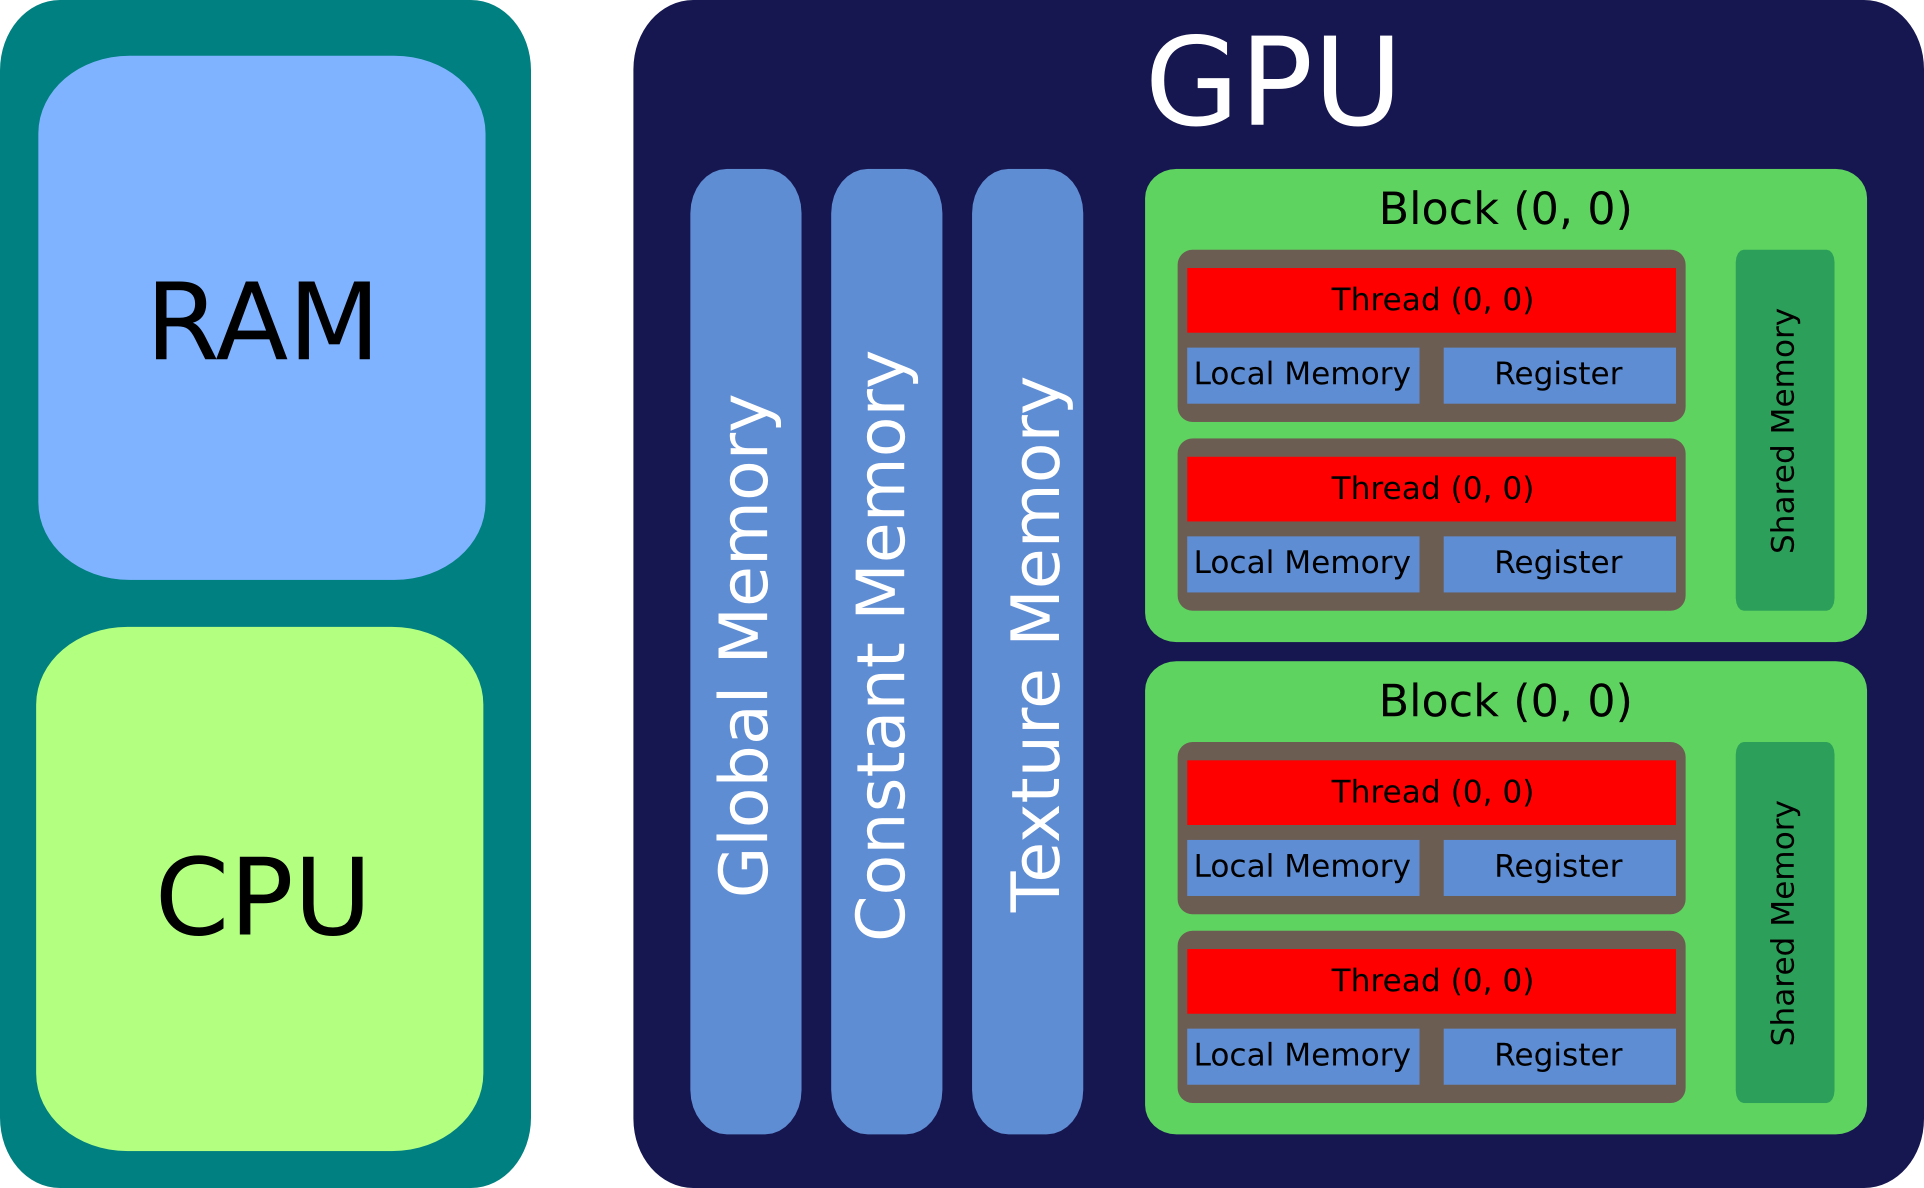
\includegraphics[width=0.8\textwidth]{gfx/cuda/gpu.png}\label{fig:gpu_arch}
  \caption{Speicherlayout einer Nvidia-GPU}
\end{figure}

-bild
-speicher bereiche
-grid layout function call
-threadidx etc

\section{Algorithmus}
-oder so ?
-erläuterung  implementierung
-speicherverwaltung

\section{Optimierung}
- coalesceded
- bank conflicts?
- teilvolumen nicht rechnen

\section{Validierung}
- beispiel rayleigh benard system
- masa
- vgl o2 vs o4 masa cube
- bifurcation


\newpage



\chapter{Immersed Boundary Methods for No-Slip Walls}
\section{Overview of Immersed Boundary Methods}

\begin{figure}[!bp]
  \centering
  \subfloat[cartesian grid]{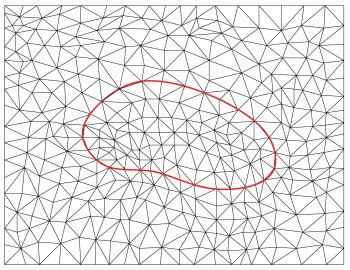
\includegraphics[width=0.4\textwidth]{gfx/immersed_boundary/general_partition_triangle.jpg}\label{fig:grid_f0}}
  \hfil
  \subfloat[unstructured body-fitted grid]{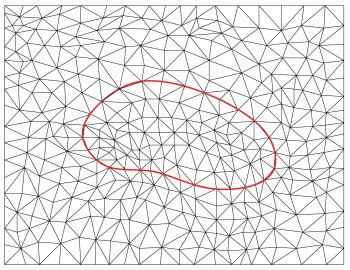
\includegraphics[width=0.4\textwidth]{gfx/immersed_boundary/general_partition_triangle.jpg}\label{fig:grid_f2}}
  \caption{Different types of numerical grids}
\end{figure}

For many fluid problems it is mandatory to solve the equations of motion with respect to complex-shaped geometries \.
The algorithm introduced in section () is not yet suitable for such a scenario.
For instance the simulation inside a spheric geometry is impossible, since the boundaries
do not coincide with the implemented cartesian grid. Nevertheless there exist different approaches to overcome this problem,
which shall be introduced here. \\
The common approach to extend the algorithm would be to use a body-fitted mesh (see figure \ref{fig:grid_f1}),
different advantages and disadvantages arise with this kind of implementation (see \citep{Mittal2005}).
One benefit is a much simpler deployment of the desired boundary condition, due to the overlap of the grid with domain border.
Furthermore a higher accuracy can be achieved \citep{Gornak2013}.
However, using an unstructered grid generates plenty of computational overhead, during and before the execution of a simulation.
The generation of the grid is very complicated in contrast to using a cartesian grid, this can be even more complicated when
considering moving boundaries.
Also solving the finite differenc schemes on a curvilinear coordinate system, leads to more calculations on a single grid point.
The last important aspect is the implementation on the gpu.
Like discussed in section () it is more efficient to use homogenous storage and calculation pattern on a CUDA-device,
the use of unstructured data makes this very difficult.
Altough some attempts exists to solve these difficulties (see i.e. PAP), it is still uncertain if the obtained performance loss would be acceptable.\\
A set of alternative methods, to resolve the problems described above, are so called Immersed Boundary Methods.
The term was first mentioned in (PESKIN 1972), for the simulation of blood flow through a heartvale, but has since then been used for a variety of
methods (MITTAL).  All of them have the idea in common to perform the simulations on a cartesian grid which does not conform to the domain boundary.
To satisfy the desired boundary conditions additional terms are introduced into the equations of motion.
In general one can distinguish between contiuous forcing methods and direct forcing methods.
Continious forcing methods try to mimic the boundary using a localized force which acts on the boundary,
since the surface is tracked by lagrangian points this methods can be well suited for moving boundaries (MITTAL).
One common problem is that continous forcing can arise to stability problem and numerical oscillations in numericial stiff problem (SOURCE).
The direct forcing approach tries to satisfies the boundary condition, by imposing it directly to points near the fluid surface for example
trough an interpolaltion procedure.
Some of the major drawbacks using the IBM is the loss in  spatial accuracy at the boundary, therefore it can be necessary to use a higher grid resolution
compared to a body-fitted mesh.  Futhermore the non-conforming (?) boundaries are more difficult implement.
The benefits of these methods is the use of a cartesian grid, which is much more suited for a gpu-based implementation (see section X).
As a result the overall performance will probably be in the same order as the original algorithm.
In the thesis the Implementation of different Immersed Boundary Methods is seperated into three chapters depending on the boundary condition and application.
This chapter beginns with Implementation of NoSlip-Walls which are the easisest to implement.
The term Immersed Boundary Method is vaguely defined in literature, in this thesis we refer to it with all methods introduced in the following three chapters.


\newpage

\section{Implemented Methods}

For the purpose of discussion, the different methods introduced here, will be applied to a default geometry.
The fluid domain without any immersed boundaries is set to a cube of the size $l_i= 1$ with  $i = \{x, y, z\}$.
For the discretization we choose $N_i = 32$ for the number of grid points.
As an example of an immersed boundary, we will dicuss the embedding of a cylinder, given by the  surface equation

\begin{align}
    \left(x - \frac{l_x}{2}\right)^2 + \left(y - \frac{l_y}{2}\right)^2 = r^2
\end{align}

where $r=0.4$ is the radius and the center is given by $(l_x/2, l_y/2)$. The whole setup is schematically shown in figure (X).
The simulation domain is than seperated into the fluid domain $\Omega_f$ and the wall domain $\Omega_w$.
The overall goal is to enforce the no-slip condition $\vec{v} = 0$ on the surface $\partial \Omega_f$, furthermore
the consveration of mass should be fulfilled.

\subsection{Volume Penalization}

\begin{figure}[!b]
    \subfloat[Cylinder geometry of the immersed boundary embedd in the simulation domain]{{
      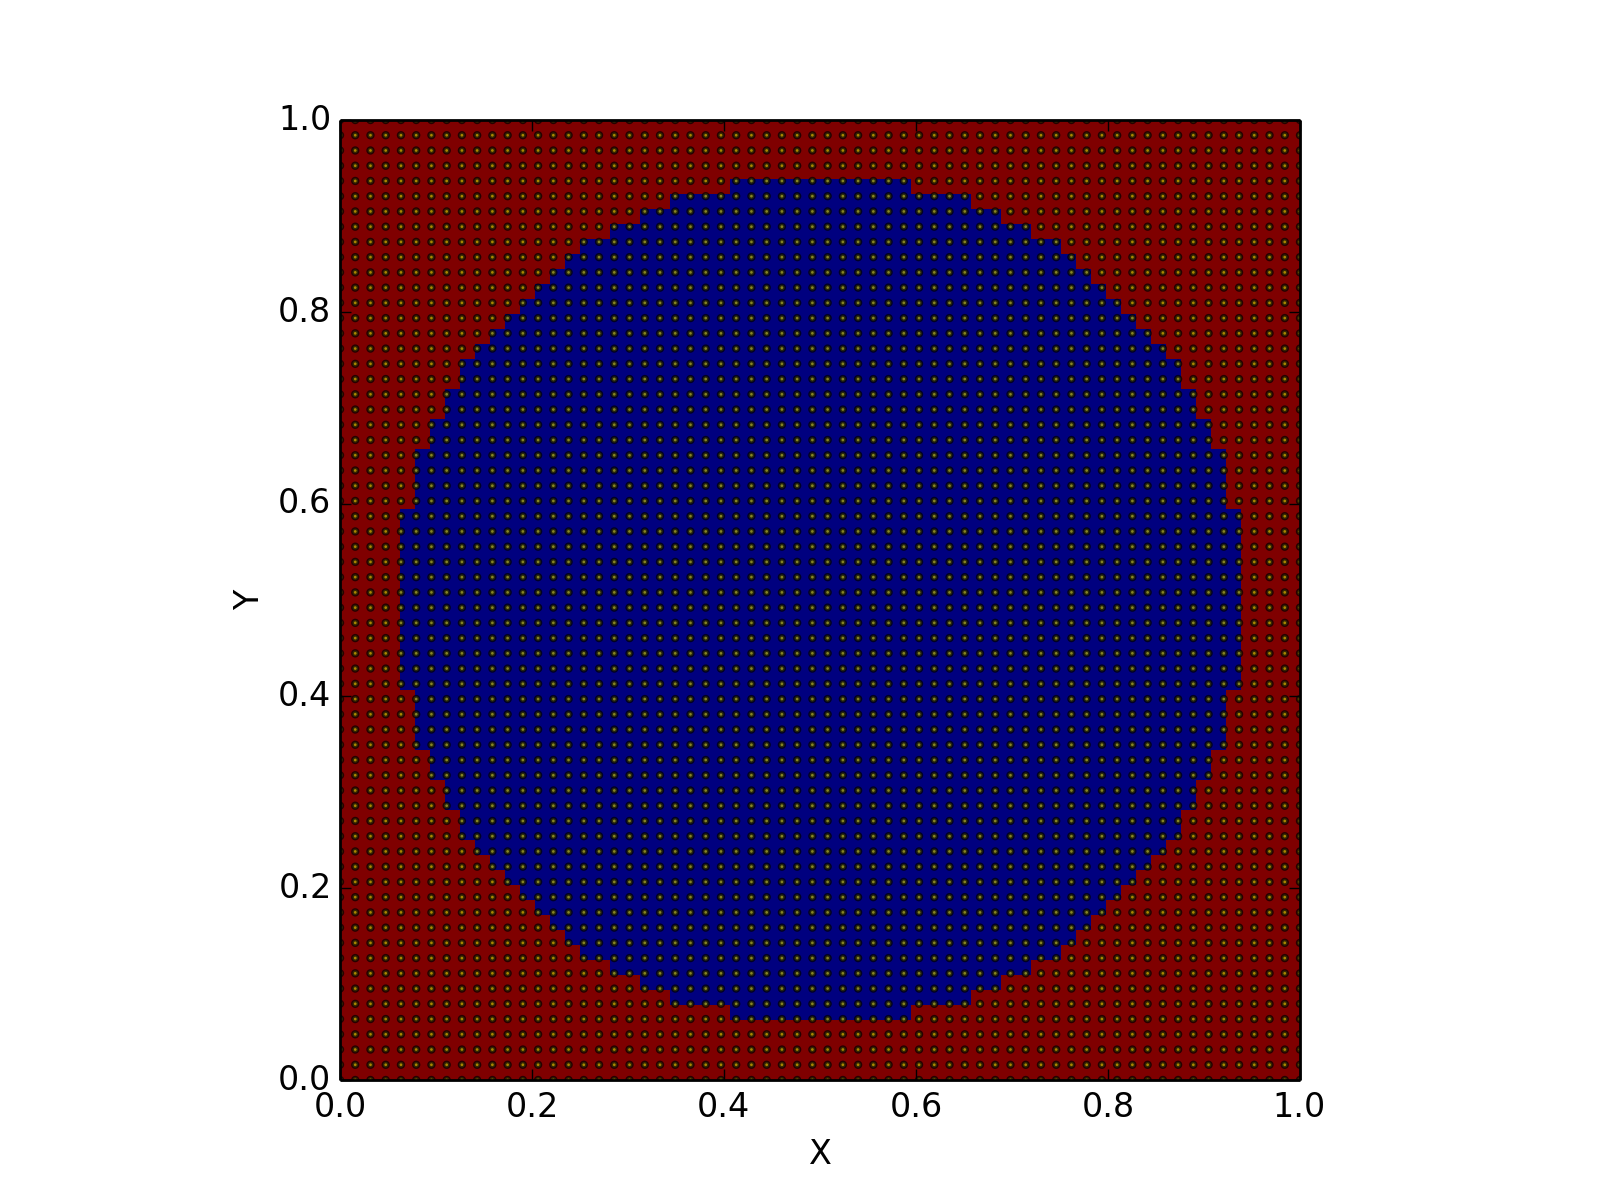
\includegraphics[width=0.5\textwidth]{gfx/immersed_boundary/mask.png}\label{fig:mask_vp}
        }}%
    \subfloat[Masking function $H(x,y,z=const.) = x^2 + y^2 < c$ for a cylinder. ]{{
      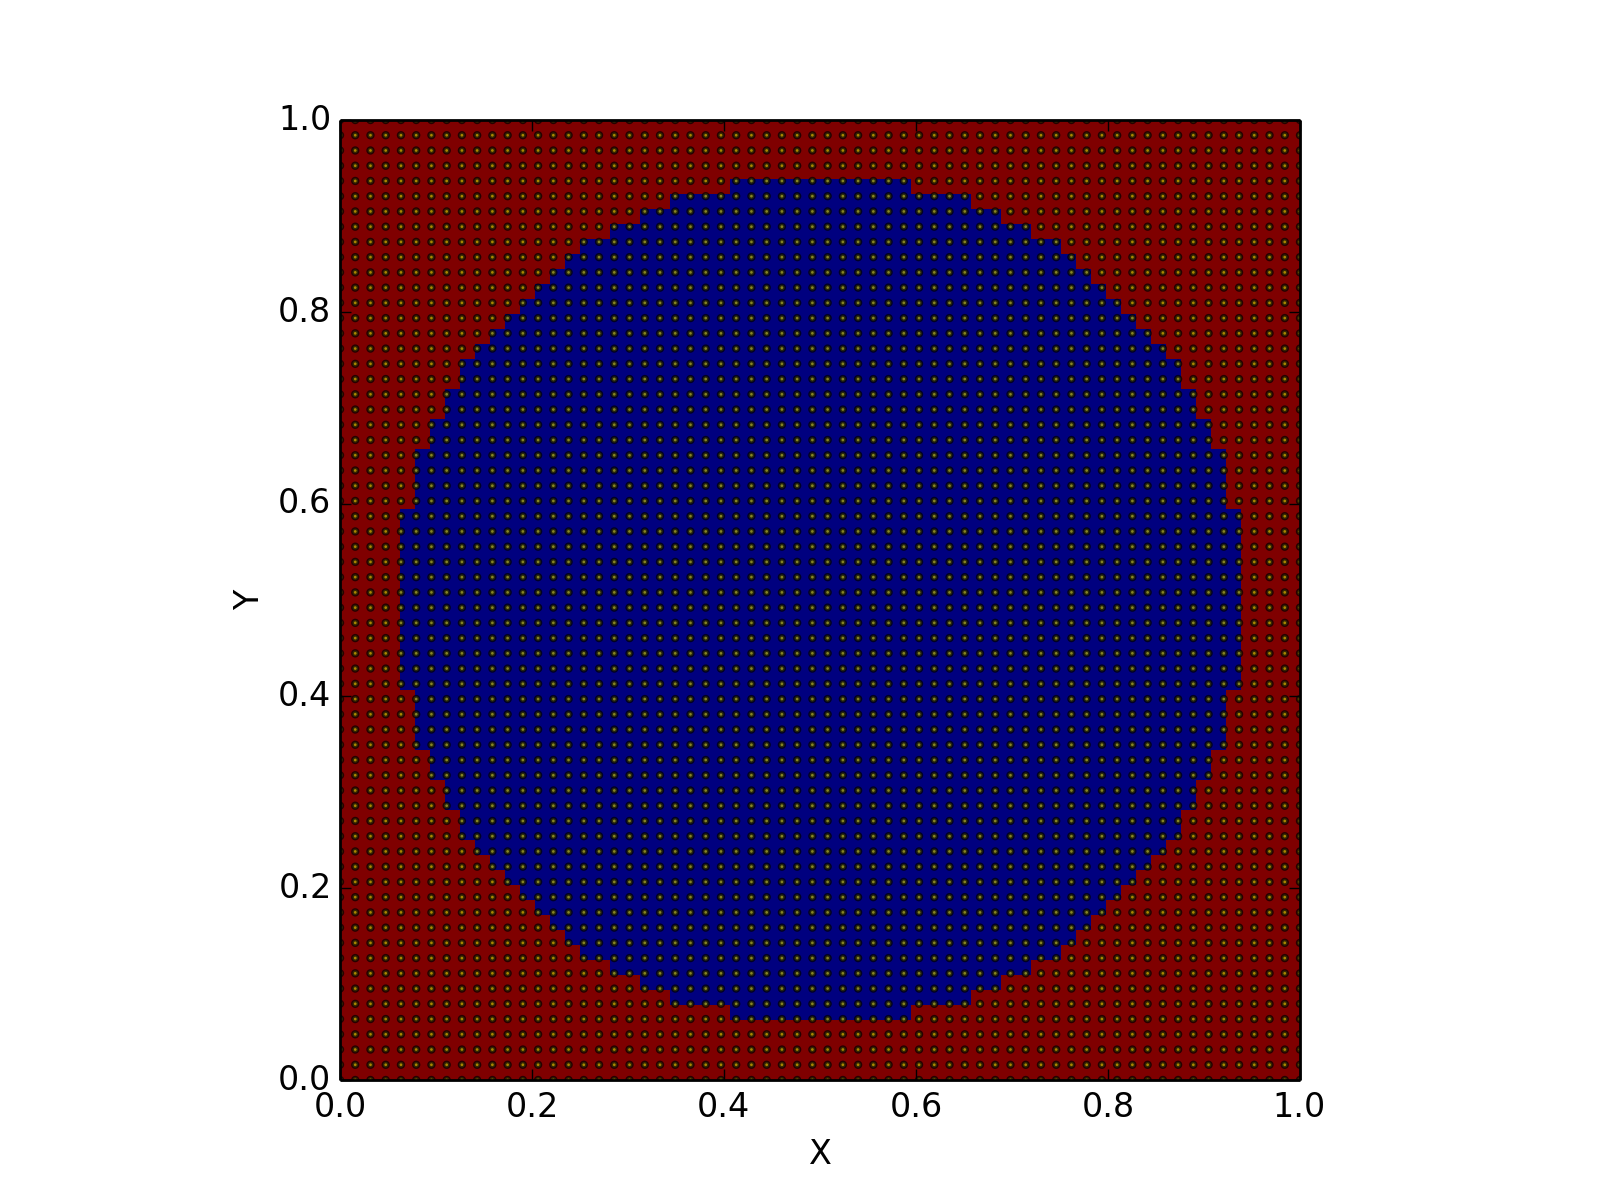
\includegraphics[width=0.5\textwidth]{gfx/immersed_boundary/mask.png}\label{fig:mask_vp}
     }}%
    \label{fig:example}%
\end{figure}

The idea behind the volume penalization method is to introduce an additional forcing term into the Navier-Stokes equation, which acts on
the grid points outside of the fluid domain to ensure the desired boundary conditions. The methods was sucessfully implemented and tested
on pseudo-spectral methods, see for example (CITE).
For the implementation it is necessary to define a masking function $H(x, y, z)$ which seperates the simulation domain into $\Omega_f$ and $\Omega_w$.
In case of the cylinder, we can use the surface equation (REF) and simply obtain.
\begin{align}
H(x, y, z) = \begin{cases}
                    0, &  \left(x - \frac{l_x}{2}\right)^2 + \left(y - \frac{l_y}{2}\right)^2 <r^2\\
                    1, & \text{else}
             \end{cases}
\end{align}
Now we can introduce an additional forcing term into the impulse equation,
\begin{align}
    \pdn[u]{t} + \vec{u} \cdot \vec{\nabla} \vec{u} &= -c^2 \nabla \rho + \frac{1}{Re} \Delta \vec{u} + \vec{F}_{ext}
     +\underbrace{ \frac{H(x, y, z)}{\nu}(\vec{v} - \vec{v_0})}_{\text{damping force}}
\end{align}

where $\vec{v}_0$ conforms the desired boundary condition, i.e. $\vec{v}_0 = 0 $ for no slip boundaries, and $\nu$ is a regulation parameter also denoted as damping rate of the forcing.
The additional term acts as an exponential damping force on a single gridpoint inside of $\Omega_w$, by the product with since it vanishes in $\Omega_f$ by the definition of $H(x,y,z)$.


Die Antwort des Kraftterms wird durch die Dämpfungrate $\nu$ reguliert. Je kleiner $\nu$ desto stärker ist die Dämpfungsrate, allerdings kann der Term
nicht beliebig klein gesetzt werden da die Stabilität für $\nu < dt$ nicht mehr gewährleistet ist [source].
Da für die Lösung der der Geschwindingskeitsfelder mit der Methode der künstliche Kompressibilität  bereits ein sehr kleiner Zeitschritt verwendet wird (s.Abb. X)
kann im Vergleich zu anderen Verfahren wie z.B. (pseudo-spektrale) eine relativ starke Dämpfungsrate verwendet werden.
-konvergenz nu gegen 0 MPI\\
- stiff probplem dt < dtpen = nu DIPLOM\\
- dary type law MPI\\
\newpage


\subsection{Direct Forcing}
Während die Volume Penalization Methode die Geschwindigkeit ausserhalb des Volumens nicht vollständig auf Null setzt,
 kann dies durch eine implizite Berechnung des Dämpfungsterm erreichtwerden. Es stellt sich heraus das dieser Ansatz equivalent
  zu der Direct Forcing Methode ist, die erstmals von [] verwendet und in [] beschrieben wird.
Betrachten wir zunächst den diskretisierten Zeitschritt
\begin{align}
    \frac{\vec{u}^{n+1} -\vec{u}^n}{\Delta t} = \mathscr{L} + \vec{f}\\
\end{align}
wobei $\mathscr{L}$ den diskretiesierten Operatoren der PDE entspricht.
Für einen Punkt auf dem Rand des Volumens soll nun die Randbedingung $\vec{u}^{n+1} = \vec{u}_0$ eingehalten werden.
Mit Formel () folgt
\begin{align}
    \frac{\vec{u}_0 -\vec{u}^n}{\Delta t} = \mathscr{L} + \vec{f} \Rightarrow \vec{f} = \frac{\vec{u}_0 -\vec{u}^n}{\Delta t\cdot \mathscr{L}}\\
\end{align}

Mit der Annahme dass der Rand mit dem numerischen Gitter übereinstimmt ist es nicht nötig den Kraftterm zur berechnen, stattdessen lässt sich der
Schritt vereinfachen in dem der Randwert nach  jedem Zeitschritt direkt auf die gewünschte Randbedingung gesetzt wird. Durch die
implizite Behandlung kommt es zu keiner weiter Stabilitätsbedingung.

\newpage

\subsection{Volume Fraction Interpolation}

The methods introduced up to here lack the ability of an exact impementation of the boundary conditions on $\Omega_f$.
Instead the surface $\partial \Omega_f$ is described by the nearest grid points in $\Omega_w$, resulting in an
stepwise approximation.
To overcome this problem a simple procedure is the use of an volume fraction interpolation scheme, introduced in [FADL].\\
The advantage of this method is the simple implementation into the volume penalization and direct forcing method.
Furthermore the overall computation time of the timestep stays constant, in  contrast to complex interpolation schemes.\\
Initially the interpolation beginns by determine all grid cells\footnote{definition cell} which are cut by the surface $\partial \Omega_f$.
For each of these boundary cells the total volume $V_w$ of the wall domain $\Omega_w$, inside each cell, is computed.
The force acting on the points inside the boundary cells is than weighted by a scaling factor, $\Phi = V_W/(\Delta x \Delta y \Delta z)$.
For the volume penalization method the scaling is simply multplied with the forcing term in eq. ().
Since the implementation of the direct forcing method is setting the velocity components directly to zero, it is necessary to
fall back to equation () and introduce a forcing term

\begin{align}
    \vec{f} = \Phi \frac{\vec{u}_0 -\vec{u}^n}{\Delta t\cdot \mathscr{L}}\\
\end{align}

\begin{figure}[!bp]
    \centering
    \subfloat[label 1]{{
      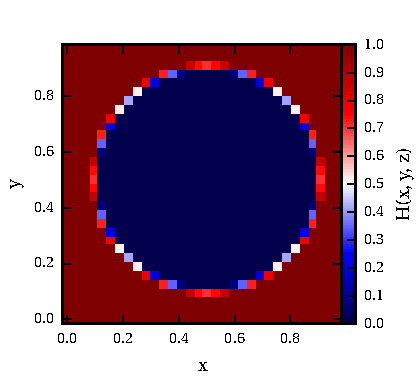
\includegraphics{gfx/immersed_boundary/methods/mask_volfrac.pdf}\label{fig:mask_volfrac}
        }}%
    \qquad
    \subfloat[label 2]{{
      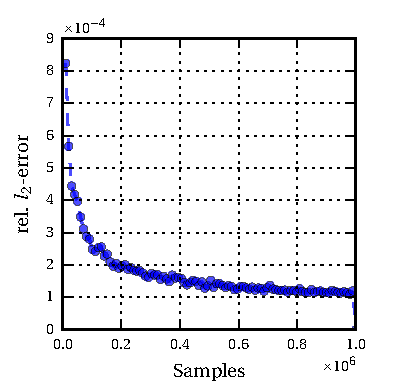
\includegraphics{gfx/immersed_boundary/methods/error_volfrac.pdf}\label{fig:error_volfrac}
        }}%
    \label{fig:example}%
\end{figure}

Since the operator $\mathscr{L}$ is computed during the first part of the time step. This forcing term can added during the completion of the runge kutta step.\footnote{see section}\\
For the implementation of an extended version of the masking array $H$ is used.
Like in the previous methods the masking array is precomputed and loaded at runtime. The algorithm is extended to compute the
volume fractions of the cells lying next to the surface $\partial\Omega_f$.
Since an exact computation is difficult to implement for abritary surfaces, the idea is to use a monte carlo integration method.
For each cell $N$ random samples are generated, then the volume fraction is simply given by the ratio of samples lying in- and outside ot the domain.
The implementation into a simulation class using the python API is explained in more detail in Appendix ().\\
An example for the computed masking array with $N=2e5$, is shown in figure (). The symmetric distribution of the boundarie values indicates
a good approximation, for a better evaluation a convergence study was performed were the number of samples $S$ was varied between 100 and $10^6$ points.
The $l_2$-error was determined by comparing the results to the computation with the highest number of samples.
The results are shown in figure ().\\

-discussion for n>10000 error 1e-5\\
-overall good approximation \\
-erweiterung  *2 etc blabla\\



\subsection{Interpolation}
\newpage

\section{Validation}

In order to ensure a correct numerical behaviour of the introduced methods,
a large part of the thesis deals with the numerical validation.
Multiple examples from simple to more complex testcases are introduced in this section.
In general it is necessary to obtain a good evaluation of the numerical truncation error, the numerical stability over longer periods of time
and the fullfilment of the conversation laws, most importantly mass conservation.
Grid convergence studys against theoretical and high-resolution numerical solutions  will be performed
and compared for the different IBMs.


\subsection{Laminar Poiseuille-Flow}
\subsubsection{Theoretical description}

\begin{figure}[!bp]
  \centering
  \includegraphics[width=0.8\textwidth]{gfx/immersed_boundary/val_volpen/poiseuilleflow.png}\label{b}
  \caption{Theoretical setup of the poiseuille-flow channel.}
\end{figure}

%\begin{wrapfigure}{r}{0.5\textwidth}
%  \begin{center}
%      \includegraphics[width=0.48\textwidth]{gfx/immersed_boundary_methods/val_volpen/poiseuilleflow.png}
%   \end{center}
%          \caption{ paxvleb xvle}
%\end{wrapfigure}


The first testcases is the laminar poiseuille-flow, the theoretical setup is presented in figure ().
It consist of two infintiy long planes at $z=h_1$ and $z=h_2$, which are oriented parallel to the xy-plane and the distance $\Delta h = h_2 - h_1$ between them.
Numerically this is realized by using periodic boundaries in xy-direction and no-slip boundaries in z-direction.
The velocity profile results from an external force, given by a  pressure gradient in x-direction, which is introduced into the naviers-stokes equation.
No other forces are present furthermore the flow will be independent of the y coordinate,
hence for the steady state $\partial v_x /\partial t = 0$ the equations of motion can be reduced to:

\begin{align}
\frac{\partial v}{\partial t} &= - \frac{\partial p}{\partial x} + \nu \frac{\partial^2 v_x}{\partial z^2} = 0
\end{align}

where v is the velocity in x direction.
For the non-dimenzionalization we choose $r^* = r/L$, $v^*=v/L$, $t^* = \frac{V}{L}$ and $p^* = p \rho V^2$ where $L=\Delta h$ and $V=v_{max}$.
The non-dimensional equation reads

\begin{align}
\frac{\partial v}{\partial t} &= - \frac{\partial p}{\partial x} + \frac{1}{Re} \frac{\partial^2 v_x}{\partial z^2} = 0
\end{align}

with $Re = VL/\nu$.
For the volume penalization method we furthermore obtain a non-dimensional damping force $-\frac{H}{J}\cdot v$ with $J = VL/\eta$.
The equation can simply be integrated twice which yields the solution

\begin{align}
v &= \frac{1}{2}\frac{\partial p}{\partial x}z^2 + zc_1 + c_2
\end{align}

Using the noslip-boundary condition $v_x(h_1) = v_x(h_2) = 0$ and furthermore by defining
$A:=\frac{1}{2}\frac{\partial p}{\partial x} Re$ one obtains the additional conditions

\begin{align}
c_1 &= A\frac{h_1^2 -h_2^2}{h_2 - h_1} = -A(h_1+h_2)\\
c_2 &= A(h_1(h_1 + h_2) - h_1^2) = Ah_1h_2\\
\end{align}

The velocity is than given by the quadratic function

\begin{align}
v_x &= A(z^2 - z(h_1 + h_2) + h_1h_2)
\end{align}

The maximum velocity and postinon can be obtained by simple calculus

\begin{align}
z_{max} &= \frac{h_1+h_2}{2} \wedge v_{max} = A\left(h_1h_2 - \frac{(h_1 + h_2)^2}{4}\right)
\end{align}

Since $v_{max}$ has to be 1 by definition of the non-dimensionalzation we find

\begin{align}
\frac{\partial p}{\partial x} &= \frac{2}{Re}\frac{1}{\left(h_1h_2 - \frac{(h_1+h_2)^2}{4} \right)}
\end{align}

as a necessary condition for the pressure gradient.\\
With the given theoretical solution, the next objective is the comparison
to the default implementation, the volume penalization method and the direct forcing method.
Since we have a flow parallel to the grid  it does not make sence to compare it to the interpolation methods
For the comparision with a theoretical solution it is necessary to ensure that the surface grid points match with the total height $h$ of the channel.
In the default setup tes gibthe noslip-boundaries are realized with the default implementation, like explained in section ().
For the immersed boundary methdos the upper- and lower boundaries are given by the masking function.
\begin{align}
H(x, y, z) = \begin{cases}
                    0, & \text{for \  }  z < h_2 \lor z>h_1 \\
                    1, & \text{else}.
             \end{cases}
\end{align}

\subsubsection{Test of the Default Implementation}

\begin{figure}[!bp]
    \centering
    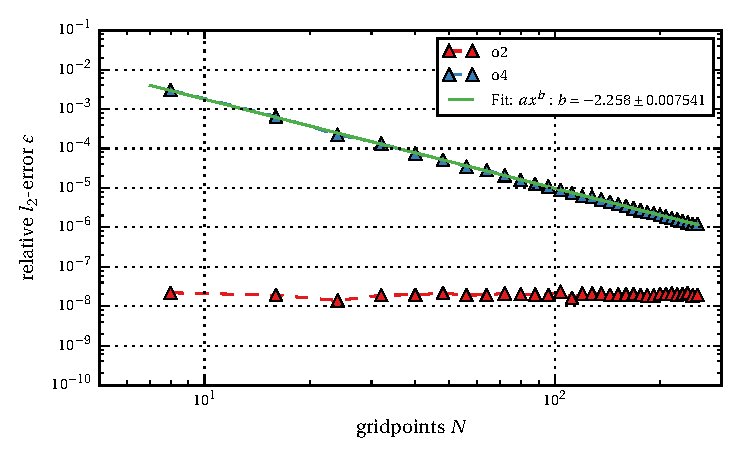
\includegraphics{gfx/immersed_boundary/poiseuille_flow/1_default/relative_l2error.pdf}
    \caption{Relative $l_2$-error for second and fourth order schemes of the default algorithm.\label{fig:ema1}}
\end{figure}

Initially a grid convergence test was performed with the default implementation of the algorithm, without the use of immersed boundaries.
For this test case this is still possible since the geometry is non-curved and parallel to the cartesian grid.\\
For the  numerical setup the parameters were set to $l_x=1$, $l_y=0.25$, $l_z=1$.
The reynolds number was set to a constant value of $Re=500$, whereas the resolution $N$ was varied in the Intervall $[16 - 128]$ with a stepsize of $\Delta N = 8$.
The timestep was set to $\mathrm{dt}=1e-5$ and the pressure gradient to $\partial p \partial x  = 10$.
For all resolutions the simulations were performed for finite differcen schemes of second and fourth order.
The results are shown in figure \ref{fig:ema1} on a double logarithmic plot.\\
For the finite difference scheme of second order, the error behaves not as assumed.
Instead of the decline one would expect with the decrease of the resolution, the  error is nearly constant.
This behaviour can be explained due to the lack of complexity of the test case. As the theoretical solution is a polynom of second order
no higher order terms will occur in the numerical solution, hence the second order scheme is capable of a perfect approximation, independent of the
grid resolution. The remaining error terms, are of the order $10e^{-8}$, which is extremly small and occur due to the floating point round off.
With this in mind the behavior of the fourth-order scheme is even more unexpected.
We see a linear decrease of the error on the log scale.
The result of a power law fit yields a convergence rate of second order.
Furthermore the error is much larger compared to the second order scheme, there is a decrease from $10e^{-2}$ to $10e^{-5}$.
The test case reveals that an error exists in the default implementation of the boundarie conditions.
An explanation can be given with comparison of the theoretical solution. The laplace operator is given by
 $ \nu \pdn[^2 v_x]{x^2} = 2A = \frac{1}{\nu}\pdn[p]{x}$
Using the mirroring method creates a discontinuous function at the boundaries, since the laplace operator changes the sign.
When using the second order method the tree-point-stencil evaluates to the correct value $\pdn[^2 v_x]{x^2} = 1$.
The five-point-stencil of the fourth orderer scheme evaluates to $\pdn[^2 v_x]{x^2} = 1$, since it uses one point behind the boundary.
As a result the discontinuity creates an error in the higher order scheme.\\
For this testcase the second order method yields better results, however we
have to keep in mind that the testcase yields a polynomial solution,
it is not clear how the results will end up for a complex testcase.
Furthermore in this testcase the boundaries have a large impact since the pressure gradient is parallel to wall,
his is not the case in general.
One possibility to avoid this error, would be to use an asymmetrich stencil, this approach is discussed in section ().

\begin{figure}[!b]
  \centering
  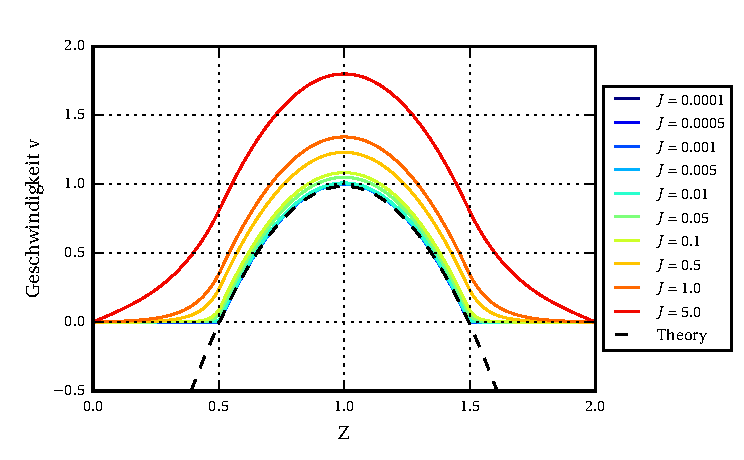
\includegraphics{gfx/immersed_boundary/poiseuille_flow/2_vp/vp_profile.pdf}\label{fig:vp_flow}
  \caption{Geschwindigkeistprofile im Kanal bei Variation der Dämpfungskonstante $\nu$ und Reynoldszahl $Re=500$.}
\end{figure}

\subsubsection{Test of the Volume Penalization Method}

The next objective is to investigate the error of the volume penalization method.
For this method the additional forcing term REFHERE is introduced into the equations. The non-dimenzionalzation leads to the form
\begin{align}
    \vec{f} = \frac{H}{J}v
\end{align}

with the quantity $J = 123$ as a non-dimensional forcing parameter.
(MACH NUBMER DISCUSSION HERE) \\
We begin by studying the behavior of the velocity profile, with variation of the Reynolds-number and the damping $J$, in the regime $Re=100-500$ and $\nu=1e-4 - 5e-1$.
The numerical setup is equal to the one for the default methods, except we now introduce the masking function (LABELABOVE) with $h_1=0.25$ and $h_2=0.75$.
To make sure that the channel width is equal to $\Delta h = 1$, the total height was set to $l_z\approx2.01587$. This furthermore ensures that the grid points overlap exactly
with the masking function at $h_1$ and $h_2$. The resolution was set to $N_x\times N_y\times N_z = 64\times16\times128$.
The resulting velocity profile is exemplarily shown in figure \ref{fig:vp_flow}, for varying $\nu$ and a constant reynolds number $Re=500$, for the second order scheme.\\
It can be noted that with an decrease of $\nu$, the numerical solution converges against the theoretical one.
The quadratic part of the velocity profile inside the fluid domain is independent of the damping constant $\nu$.
Since the damping can not fullfill the exact boundarie conditions, a slight offset is introduced into the velocity profile
which leads to an offset in the solution.
In the masked area of the volume we can see an exponential decrease of the total velocity.
Since for the steady state

\begin{align}
 \nu v &= D \frac{\partial^2 v_x}{\partial z^2}  \Rightarrow  v_x = A e^{\sqrt{\frac{\nu}{D}}v_x}
\end{align}

where A is given by the offset $v(h_1)$.\\
For an error estimation, the relative $l_2$-error was computed.
The results for the second order scheme are shown in figure \ref{fig:vp_error}.

\begin{figure}[!t]
  \centering
  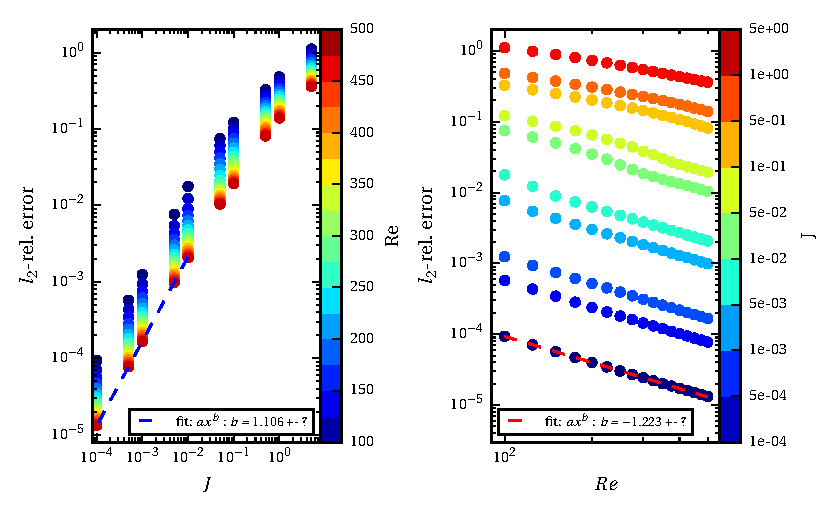
\includegraphics{gfx/immersed_boundary/poiseuille_flow/2_vp/vp_error.pdf}\label{fig:vp_error}
  \caption{Relative $l_2$-error for variable damping rate $\nu$ and reynolds-number $Re$.}
\end{figure}


The error decreases together with the damping rate from $1e-0$ to $1e-4$. For $nu<1e-3$ and a constant reynolds number we can observe an almost linear decrease in the logarithmic space,
this yiels a fit law of the form $ e = ax^b$. This shows that the error of this penalization method converges with first order in dependence of $\nu$.
The decrease for $nu>=1e-3$ can be explained by having a look at figure \ref{fig:vp_flow} again. Since the damping in the masking area is to
weak the flow sees the real boundaries of the fluid domains, which results in a stronger damping on the flow.
This is not the case for $nu<1e-3$ since the velocities reaches zero before reaching the boundarie.\\
Furthermore we can see a decrease of the error of one order with an increase in the reynolds number.
Since the damping force is proportional to the velocity and therefore to the reynolds number, the offset on the channel walls remains constant.
Due to the larger velocity profile this results in an smaller relative $l_2$-error, whereas the absolute error will increase.
For the fourth order scheme, the error is shown in figure APPENDIX.
We can observe a similar convergence  until the damping rate decreases to $\nu=1e-4$, below that value the error increases slightly to the order of magnitude of $1e-3$.
The reason for this behavior will be discussed soon.\\
Finally a grid convergence study was carried out, with a constant Reynolds number and $\nu \in [1-23]$.
The resolution was varied between $N\in [4, 400]$ with $\Delta N = 4$, second and fourth order schemes were tested.
For the correct solution the theoretical velocity profile (REF) was assumed.
The results are shown in figure().

\begin{figure}[!t]
  \centering
  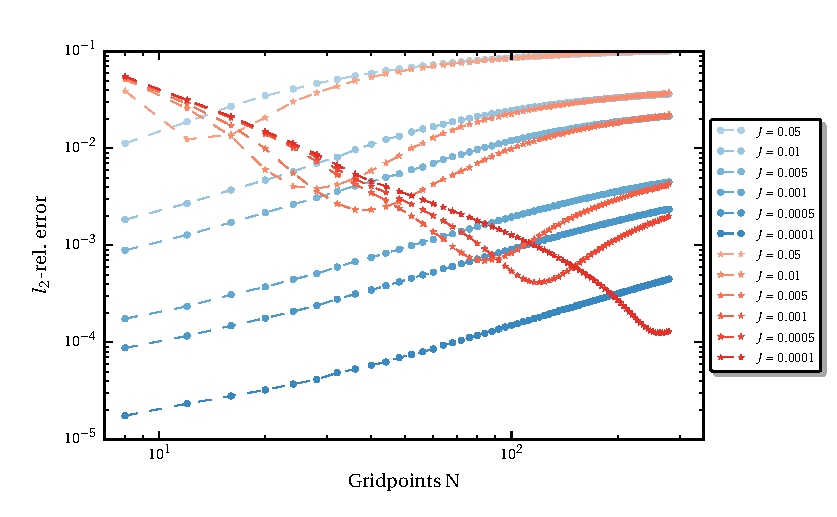
\includegraphics{gfx/immersed_boundary/poiseuille_flow/2_vp/vp_convergence.pdf}\label{fig:vp_conv}
  \caption{Absoluter und relativer Fehler in Abhängigkeit von Dämpfungskonsante $\nu$ und Reynoldszahl $Re$.}
\end{figure}
One can observe again that a decrease in $\nu$  yields a smaller error.
For the second order scheme we can see that with an increase in the resolution, the error increases and finally converges against a constant value.
Even more confusing is the behaviour for the fourth order scheme.
With increasing resolution we can see a decrease into a local minimum, followed by an increase to the same error as the second order scheme.
An explanation of this behaviour can by given by revising the theoretical solution and the finite difference stencils at the immersed boundary.

The error does not converge towards zero, which means there has to be some discrepancy to the theoretical solution.
For a constant $\nu$ there is an offset to the theoretical solution, which we allready saw in figure (REF).
Hence by increasing the resolution the numerical solution converges towards the wrong solution.
The error increases since for a lower resolution, the velocity profile is closer to the assumed theoretical for the second order method.

\begin{align}
 \nu v &= D \frac{\partial^2 v_x}{\partial z^2}  \Rightarrow  v_x = A e^{\sqrt{\frac{\nu}{D}}v_x}
\end{align}
\begin{figure}%
    \centering
    \subfloat[label 1]{{
      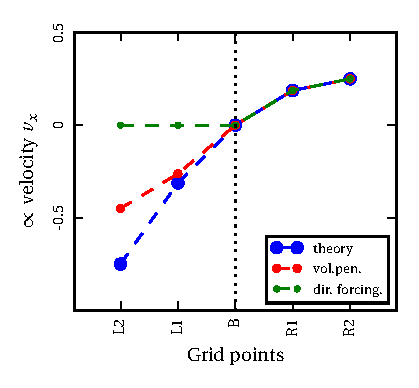
\includegraphics{gfx/immersed_boundary/poiseuille_flow/extra/stencil.pdf}\label{fig:mask_vp}
        }}%
    \qquad
    \subfloat[label 2]{{
      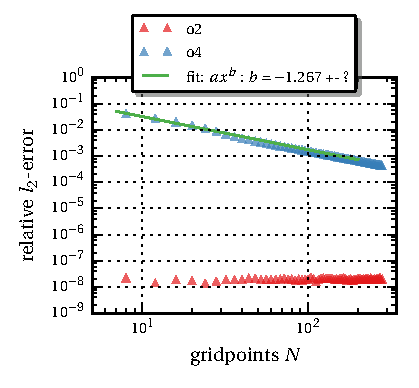
\includegraphics{gfx/immersed_boundary/poiseuille_flow/3_df/relative_l2error.pdf}\label{fig:mask_vp}
        }}%
    \label{fig:example}%
\end{figure}


The explanation for the fourth order convergence has again to do with the discretization error at the boundary.
Figure () shows schematically the velocity profiles for the volume penalizaton method compared to the theoretical.
Due to the different  profiles, the numerical evaluation of the laplace operator results
into different friction rates for the border point \textbf(B), but  also for the first next neighboor in the fluid domain \textbf(R1) when fourth order schemes are used.
For the fourth order scheme the laplace operator at the boundary evaluates to a slightly (CALCULATE) negative value), which means the friction at the boundary due to
viscosity is stronger. The result is a smaller velocity profile which when increasing the resolution starts to overlap best with the theoretical solution at the minimal error.
Finally when increasing the resolution further the error increases since the method converges towards the same resolution as the second order scheme (IMAGE MAYBE?).
An attempt has been made to fit the numerical solution to a quadratic profile for the comparision to a theoretical solution but this didn't work due to blabla
(FIT IDEA NOT WORKING CONVERGENCE AGAINST HIGH RESOLUTION.

\subsection{Direct Forcing Method}

For the comparsion to the direct forcing method another grid convergence study was carried out.  As a parameter we used same as above, the results are shown in figure X.
-We can see o4 not working reason is the same as we can se in figure n) , the laplacian is wrong caclulated at the point B.
As a results an error is induced at the boundaries of the domain.
The second order scheme works perfectly as we compare it to the default implementation.

\subsection{Poiseuille Flow with variable pressure gradient}

Finally

\begin{align}
\frac{\partial p}{\partial x} &= P_0 \sin(\pi n z)
\end{align}

solution with the same non-dimensionalization yields

\begin{align}
 \nu v &=  \sin(\pi n z)
\end{align}

with the condition

\begin{align}
 P_0 &= -\frac{\pi^2n^2}{Re}
\end{align}

to satisfie $v_{max} = 1$.


\begin{align}
 \nu v &= D \frac{\partial^2 v_x}{\partial z^2}  \Rightarrow  v_x = A e^{\sqrt{\frac{\nu}{D}}v_x}
\end{align}
\begin{figure}%
    \centering
    \subfloat[label 1]{{
      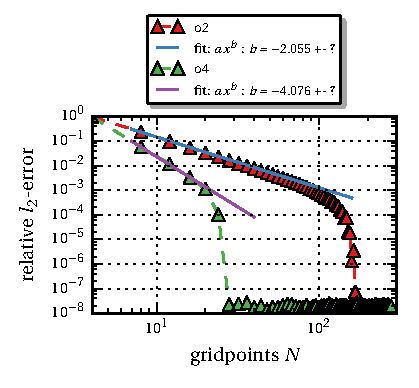
\includegraphics{gfx/immersed_boundary/poiseuille_flow/4_sine/relative_l2error.pdf}\label{fig:mask_vp}
        }}%
    \qquad
    \subfloat[label 2]{{
      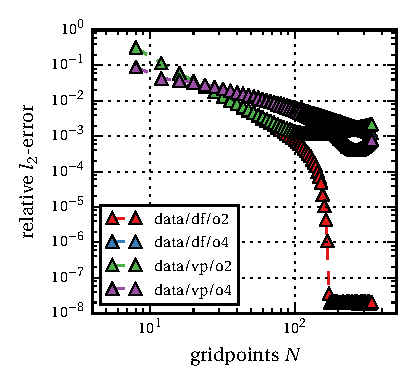
\includegraphics{gfx/immersed_boundary/poiseuille_flow/4_sine/relative_l2error_methods.pdf}\label{fig:mask_vp}
        }}%
    \label{fig:example}%
\end{figure}

\newpage
\subsection{Hagen-Poiseuille Flow}

\subsubsection{Theoretical description}

In the previous testcase the channel walls were aligned parallel to the simulation grid, hence no further interpolation procedures
were necessary. In order to test the accuray of the interpolation methods, we now introduce a testcase with a curved geometry.
Furthermore we have the possibility to investigate the error of non-interpolating methods on curved surfaces.\\
The most simplest extension of the planar poiseuille flow, is the laminar flow through a pipe,
also referred to as Hagen-Poiseuille flow. The setup of the fluid domain is schematically shown in figure ().
We consider a flow in z-Direction where the total size of the simulation domain is set to $L_x = L_y = L$.
The immersed boundary is restricted by a wall at the radius $r_0=0.4L$ where r is defined as the distance from the pipe center $\vec{m} = (L/2, L/2)^T$.
The length $L_z$ can be chosen arbitrary due to the flow invariance in z direction.\\
\begin{figure}[!bp]
  \centering
  \includegraphics[width=0.8\textwidth]{gfx/immersed_boundary/val_volpen/poiseuilleflow.png}\label{b}
  \caption{Theoretical setup of the poiseuille-flow channel.}
\end{figure}
For an analytical solution of this problem we referr to [CITEFLUID].
Once again we can assume a steady state flow which implies $\partial v_z/\partial t = 0$. With the introduction of cylindrical coordinates $(r, \phi, x)$
and the assumption that the flow is independent of $\phi$ the equation of motion reduces to
\begin{align}
        0 &= - \frac{\partial p}{\partial x}  +  \frac{\nu}{r}\frac{\partial}{\partial r}\left(r\frac{\partial u}{\partial r}\right)
\end{align}
The solution is obtained by seperation of variables and integrating twice.
\begin{align}
    u &= \frac{r^2}{4\nu}\frac{\partial p}{\partial x} + A \ln r + B
\end{align}
By using the boundarie conditions $u(r_0) = 0$ and choose the same non-dimensionalization as in section (), with the expection of setting the length scale to $r_0$,
the velocity profile for the channel is given by
\begin{align}
    u &= \frac{r^2 - r_0^2}{4}\frac{\partial p}{\partial x}Re
\end{align}
Since $v_{max} \stackrel{!}{=} 1$ by definition, the pressure condition for the domain needs to be set to
\begin{align}
    \frac{\partial p}{\partial x} = -\frac{4 r_o^2}{Re}
\end{align}

\subsubsection{Grid Convergence Study}

For an error evaluation a grid convergence study was performed, for a constant reynolds number of $Re=100$.
The number of grid points was varied in the intervall $N\in[32, 256]$ with a stepsize of $\Delta N = 16$, furthermore a
simulation with a resolution of $N=512$ was carried out.\\
Since the maximum velocity of the channel is given by $v_{max}=1$, due to the choice of non-dimensionalization,
the sound speed was set to $c^2 = 100$ to fullfill the incompressibilty condition $Ma = v/c < 0.1$. \footnote{In order to exclude
any influence of choice of the sound speed on the resulting error, further simulations were carried out with a diffent $c^2$ and will be discussed}
With this choice the cfl-condition for the system is given by $\Delta t < \min(\Delta x^2 \cdot Re, \Delta x / 10)$.
The resulting timestep for the highest resolution is $\Delta t = 1e-4$.
With the above defined setup all methods introduced in section were tested, for second and fourth order finite difference stencils.\\
For the penalization method the non-dimensionalized damping was set to $J=1e-4$.
It would be possible to choose a larger time step for the lower resolution cases, which means that in general
one would apply a smaller damping rate $J$ in a case of applicaton. To remain consistent in the error convergence, here $J$ and
therefore $\Delta t$ was not altered.\\
The results of the computation are shown from figure () to figure().
In figure (X) the relative $l_2$-error is shown for the volume penalization method with and without the volume fraction method
for second and fourth order. The modified volume fraction method is not present since the computed error is almost identical to the default method,
such that the values overlap in the plot.

\begin{figure}[!pt]
  \centering
  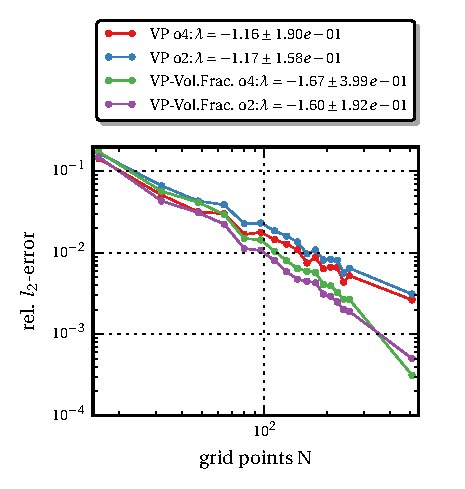
\includegraphics{gfx/immersed_boundary/hpflow/theo/vp.pdf}\label{fig:hpflow_vpgc_theo}
  \caption{blabla}
\end{figure}

\begin{figure}[!pb]
  \centering
  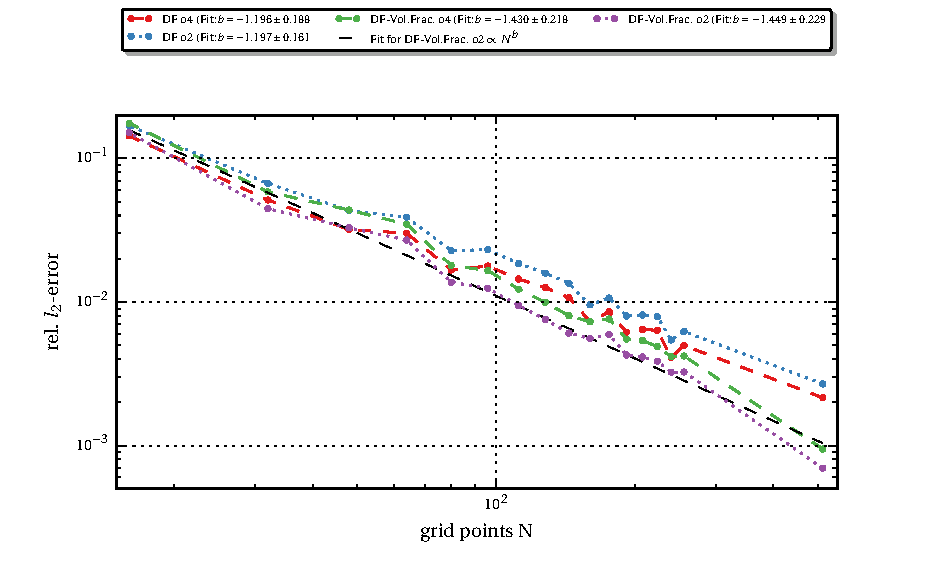
\includegraphics{gfx/immersed_boundary/hpflow/theo/df.pdf}\label{fig:hpflow_dfgc_theo}
  \caption{blabla}
\end{figure}


\begin{figure}[!pt]
  \centering
  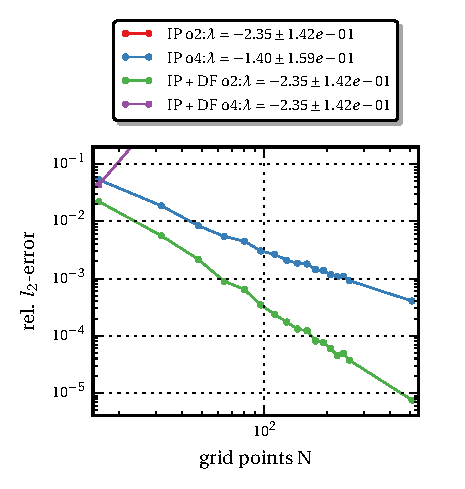
\includegraphics{gfx/immersed_boundary/hpflow/theo/ip.pdf}\label{fig:hpflow_ipgc_theo}
  \caption{blabla}
\end{figure}

\begin{figure}[!pb]
  \centering
  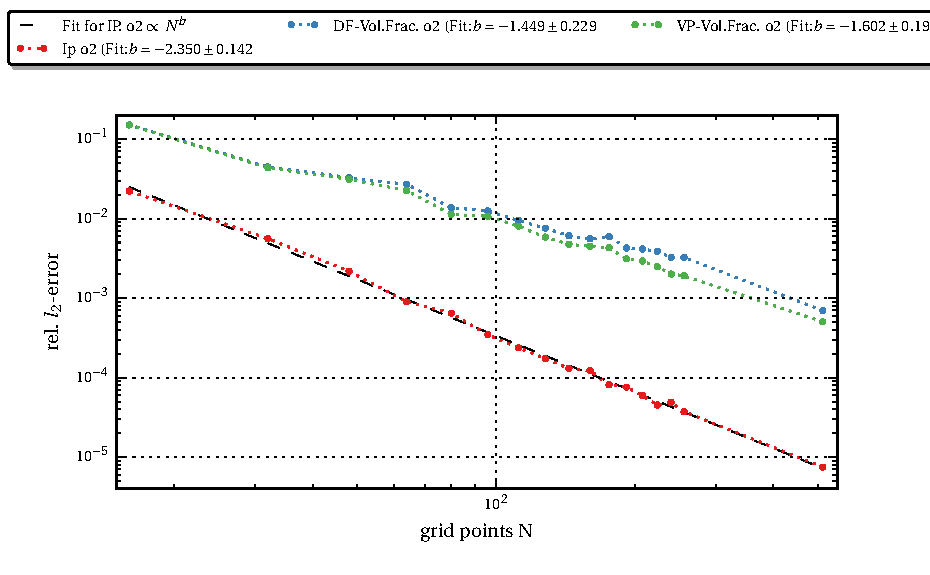
\includegraphics{gfx/immersed_boundary/hpflow/theo/all.pdf}\label{fig:hpflow_allgc_theo}
  \caption{blabla}
\end{figure}

\newpage


For all methods an approximately linear decrease  can be observed.
The error decreases from the order $1e-1$ for low resolutions until


-numerical setup resolution
-sound speed squared
-dt choice
-nu choice

-discussion c2 400

\subsubsection{Long-Term Simulations}
\newpage


\subsection{Taylor-Couette Flow}

-introduction

\subsubsection{Theoretical description}

blub blub

\newpage
\thispagestyle{empty}
\mbox{}

% \newpage
% \thispagestyle{empty}
% \mbox{}l
% %\cleardoublepage


\printbibliography

% \chapter*{Danksagung}

\begin{otherlanguage}{ngerman}
  \thispagestyle{empty}





  \null\vfill
  \noindent
\end{otherlanguage}

\end{document}
